\documentclass[12pt]{mitthesis}
\usepackage[pdftex]{graphicx}
\usepackage{subfloat}
\usepackage{kylesthesis}
\begin{document}

\tableofcontents
\clearpage

%\listoffigures
%\clearpage

\subsubsection*{NOTES}
\clearpage

\setcounter{chapter}{5}
\chapter{  IR-UV double resonance LIF/SEELEM spectroscopy of the
  $3^34^1$ \Ka{0} and $3^36^1$ \Ka{0} vibrational sublevels of $S_1$
  acetylene}

\section{Introduction}

The \AtoX\ spectrum of acetylene, \ce{C2H2}, provides a quintessential
example of an electronic transition accompanied by a change in
geometry.  The acetylene molecule is linear in the ground state ($S_0$),
but has a planar \emph{trans}-bent geometry in the \astate\ state
($S_1$) \cite{ingold, vanveen}.  \emph{Ab initio} calculations are in
agreement that all low-lying electronic excited states, singlet and
triplet, have minima in a planar \emph{trans}-bent geometry \cite{all,
  abinitio, papers}.  The sole exception is the third triplet state,
$T_3$, which instead has a minimum in a non-planar geometry, twisted
approximately 75\degrees\ out of plane from the \emph{trans}
configuration \cite{cui96, ventura03, thom07}.

Experiment and theory have shown that vibrational levels of the $T_3$
electronic state play a crucial role in allowing mixing between $S_1$
levels and the dense manifold of optically dark $T_{1,2}$ levels
\cite{humphrey97, altunata00, dupre93, cui97, thom07, ventura03}.  The
fundamental premise of the model is that spin-orbit matrix elements
between $S_1$ and $T_{1,2}$ levels are much smaller than those between
levels of $T_3$ and $T_{1,2}$.  In the doorway model, mixing between
$S_1$ and $T_{1,2}$ levels occurs as a second-order effect; a level
of $S_1$ must mix with $T_3$, which, in turn, permits mixing with the
manifold of $T_{1,2}$ levels.

% The word ``doorway'' implies that the $S_1 \sim T_3$ mixing is
% dominated by a single $T_3$ vibrational level.  Because the levels of
% $T_3$ are so widely spaced ($\sim 10$ \rcm) relative to the average
% $S_1 \sim T_3$ spin-orbit matrix element ($\sim 0.1$ \rcm), this is
% almost always the case.

The magnitude of $S_1 \sim T_3$ spin-orbit matrix elements is
controlled principally by vibrational overlap factors, resulting in
vibrational specificity for $S_1 \sim T_3$ mixing.  To date, most
studies have addressed the role of the symmetric \emph{trans}-bending
mode, partially because the levels containing this
Franck-Condon-active vibration are well understood and appear with
great intensity in the \AtoX\ spectrum.  Many studies have observed an
increase in $T_3$-mediated $S_1 \sim T_{1,2}$ mixing with increased
excitation in the $\nu_3$ (\emph{trans}-bend) vibrational mode of
\astate\ acetylene \TODO{cite}.

The role of the non-symmetric bending modes, $\nu_4$ (torsion) and
$\nu_6$ (antisymmetric in-plane bend), is much less clear.  Since the
geometry change from in-plane to out-of-plane occurs along the
torsional coordinate, a simple Franck-Condon model would predict that
increased excitation in the torsional mode ($\nu_4$) would lead to
increased $S_1 \sim T_3$ vibrational overlap.  However, the current
experimental evidence and theoretical calculations disagree with this
na\"{i}ve model.  Mizoguchi et al. observe large splittings in the
spectrum of $3^36^1$ \Ka{1}, but not in the spectrum of $3^34^1$
\Ka{1} \cite{mizoguchi00}.  Yamakita and coworkers observe Zeeman
quantum beats in several rotational lines in the spectrum of $3^36^1$
\Ka{1}, but none in the spectrum of $3^34^1$ \Ka{1} \cite{yamakita01}.
These authors cite agreement with the calculations of Cui and
Morokuma, who predict a half-linear geometry for the minimum of the
seam of intersection between the $S_1$ and $T_3$ electronic surfaces
\cite{cui96}.  Such a half-linear geometry is accessible via a
combination of the $\nu_3$ and $\nu_6$ vibrations.

We are left without explanation as to the small magnitude vibrational
overlap integrals upon excitation in mode 4, relative to mode 6.  In
an effort to address this problem, Virgo and coworkers recently
published a comparison of the simultaneously recorded SEELEM/LIF
spectrum of the $2^13^14^2$ \Ka{1} and $2^13^16^2$ \Ka{1} sublevels.
They observe that the SEELEM:LIF intensity ratio is three times larger
for $2^13^14^2$ \Ka{1} than for $2^13^16^2$ \Ka{1}.  In order to
characterize the experimental results in terms of $2^13^14^2$ and
$2^13^16^2$ basis character, they present a tentative deperturbation
of the $2^13^1B^2$ polyad, which consists of the $2^13^14^2$ ($a_g$),
$2^13^16^2$ ($a_g$), and $2^13^14^16^1$ ($b_g$) levels.  They
determine that $2^13^14^2$ and $2^13^16^2$ basis character is
essentially evenly distributed between the two \Ka{1} sublevels
observed in the experiment.  The difference in SEELEM:LIF intensity
ratio is ascribed instead to be the result of an interference effect
which cancels out almost all $2^13^14^16^1$ ($b_g$) basis character in
one of the levels.

The interference effect is due to two separate, strong interactions
between the $\nu_4$ and $\nu_6$ vibrations.  The first interaction is
a strong Darling-Dennison resonance, which connects vibrations by
exchanging two quanta of $\nu_4$ for two quanta of $\nu_6$, or vice
versa.  Levels having only one quantum of modes 4 or 6, such as those
studied by Mizoguchi, are immune to this effect.  The second
interaction is the $a$-axis Coriolis coupling, which exchanges one
quantum of mode 4 for one quantum of mode 6.  The matrix element for
$a$-axis Coriolis coupling includes a factor of $K$, thus sublevels
having $K=0$ are immune to this effect.

In this study, we seek to address the role of modes 4 and 6 in
promoting vibrational overlap with $T_3$ levels.  To avoid the
Darling-Dennison resonance, we select a polyad with one quantum of
non-symmetric bend.  To avoid \emph{a}-type Coriolis coupling, we examine
the $K=0$ sublevels of the polyad members.  To investigate the effects
of $\nu_4$ and $\nu_6$ near the crucial half-linear and twisted
geometries, we select the particular combination levels $3^34^1$ and
$3^36^1$ of $S_1$ acetylene.





























\section{Experiment}

Vibrational levels of \astate\ acetylene having \emph{ungerade}
symmetry are inaccessible via one-photon transitions from the ground
state, according to $g$/$u$ selection rules.  To access the $3^34^1$
($a_u$) and $3^36^1$ ($b_u$) levels, we employed an IR-UV double
resonance scheme.  The $\nu_3''+\nu_4''$ level of the \xstate\ state
was chosen as an intermediate state for laser excitation.  According
to the selection rule $K'-\ell'' = \pm 1$, the $K'=0$ sublevels of
$3^34^1$ and $3^36^1$ are accessible from this $\ell''=1$ ground state
intermediate.

IR laser radiation in the region of 3900 \rcm\ was generated from the
output of a tunable dye laser (Lambda Physik FL2000) operating in the
region of 740 nm.  \TODO{Provide details of IR difference-frequency
  generation and amplification.}  The IR laser radiation was
calibrated using a photoacoustic cell containing approximately 100
mTorr of acetylene.

The UV laser radiation used in the second step of the double resonance
was generated from the output of an Nd:YAG (Spectra Physics) pumped
dye laser (Lambda Physik FL3002) operating in the region of 450 nm.
The dye laser output was frequency doubled using a BBO crystal.  The
UV laser radiation was calibrated by recording the absorption spectrum
of \ce{Te2} using the fundamental frequency output of the dye laser.
The frequency step size of the UV laser was approximately 0.047 \rcm\
(frequency doubled output) in this study.

The IR and UV beams were positioned in an overlapping, colinear
geometry inside the SEELEM/LIF apparatus.  The UV laser pulse was
delayed by 10 ns relative to the IR pulse by using several UV
reflectors to create an optical delay line.  A dichroic mirror,
transparent in the IR, was used to combine the IR and UV beams.
\TODO{Look up polarization of lasers, $p$ or $s$.}

The experimental arrangement of the SEELEM/LIF apparatus has been
described previously.  \TODO{Cite.}  Briefly, the apparatus consists
of two differentially pumped vacuum chambers, a source chamber and a
SEELEM detection chamber.  In the source chamber, a supersonic jet of
acetylene gas (Matheson) is expanded from a 10 Hz pulsed valve
(Jordan).  The source chamber is pumped by a 6 inch diffusion pump
(Varian), and has a typical operating pressure of $10^{-4}$ Torr.
Approximately 2 cm downstream from the nozzle, the molecules are
excited by the overlapping UV and IR laser beams, which intersect the
axis of the jet at a 90\degrees angle.  The laser-induced molecular
fluorescence is collected by $f/4$ optics along an axis normal to the
plane defined by the lasers and the jet axis.  The fluorescence passes
through a filter (UG-11) and is detected by a photomultiplier tube
(Hamamatsu R375).  The time-varying photomultiplier output signal is
averaged at each laser frequency on a digital oscilloscope (LeCroy)
and recorded on a PC \TODO{Determine how many bits the scope has}.

Approximately 5 cm from the region of excitation, molecules in the
supersonic expansion pass through a 3 mm diameter skimmer and enter
the SEELEM detection chamber.  The detection chamber is also pumped by
a 6 inch diffusion pump (Varian), and has a typical operating pressure
of $10^{-6}$ Torr.  The SEELEM detector is positioned along the
molecular beam axis, approximately 35 cm downstream of the excitation
region.  The design of the SEELEM detector used in these experiments
has been described by several authors \TODO{cite}.  In the SEELEM
detector, electrons ejected from a grounded metal surface are detected
by an electron multiplier (ETP).  The electron multiplier output is
sent to a fast amplifier/discriminator (EG\&G/Ortec), and the
resulting pulses are acquired by PC-operated multichannel scalar
hardware.

To eject an electron from the metal surface of the SEELEM detector, an
excited molecule must have a vertical electronic excitation energy
exceeding the work function of the metal.  In this study, a gold
surface was used, having a work function of approximately 5.1 eV.
Among the low-lying electronically excited states of acetylene, only
$S_1$ and $T_3$ have sufficient energy to be detectable on gold.





















\section{Results}

The spectra in this study were collected using two double resonance
strategies: a survey method and an ``individual line'' method.  In the
survey method, the IR laser was tuned to the Q-branch head of the
$\nu_3''+\nu_4''$ level in the ground electronic state.  The Q-branch of
this band is very compact, and the incoherent linewidth of the IR
laser is sufficient to excite the rotational levels $J=1f-5f$ at a
single laser frequency.  From the $f$-symmetry rotational levels
populated in the first excitation step, Q-branch transitions in the UV
are permitted to the $3^34^1$ \Ka{0} sublevel, and P or R-branch
transitions are permitted to the $3^36^1$ \Ka{0} sublevel.  A diagram
of the energy levels and the allowed transitions is shown in Figure
\ref{fig:levels-iruvdr}.

\begin{figure}
  \centering
  
  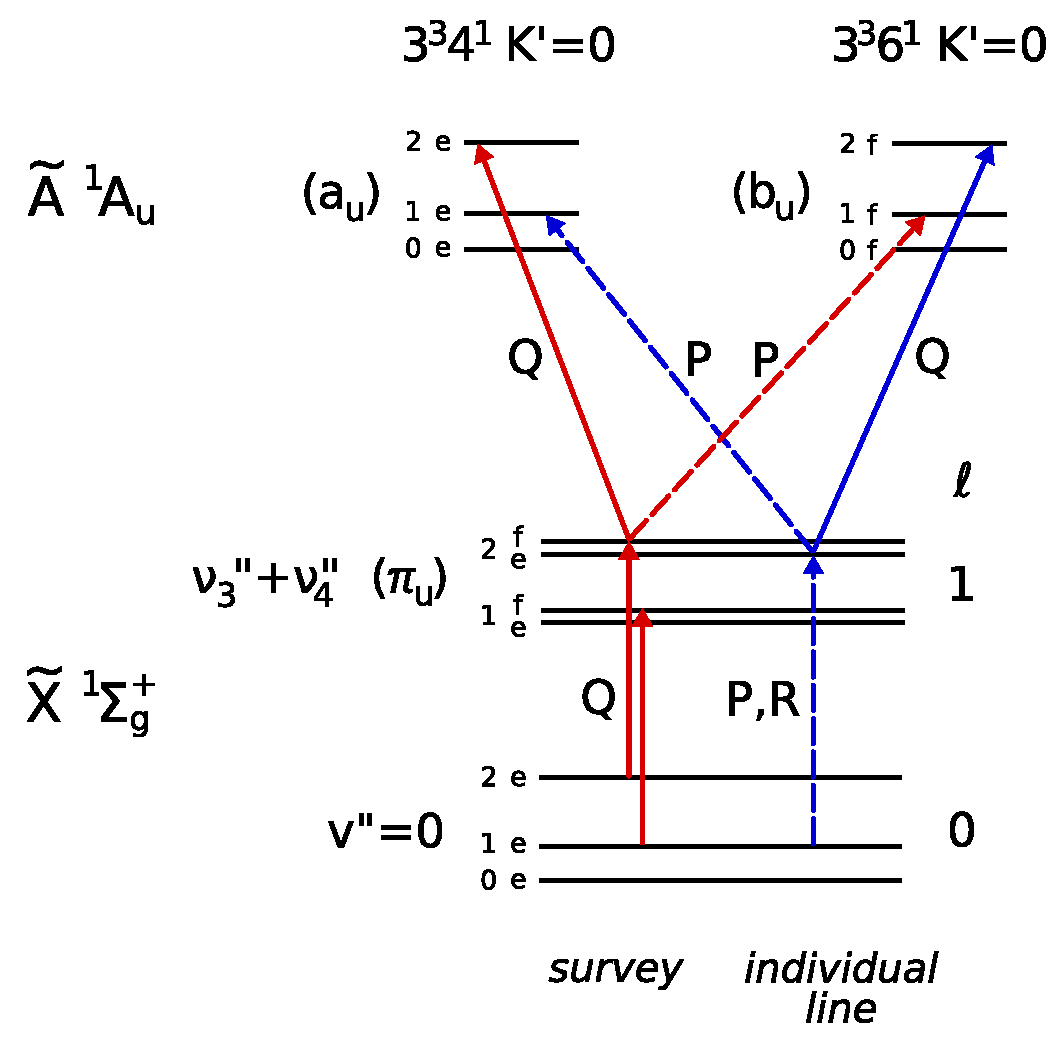
\includegraphics[width=5in]{levels-iruvdr}

  \caption{Schematic diagram of the IR-UV double resonance methods
    used in this study.  In the survey method, the Q(1)-Q(5)
    transitions terminating in the $\nu_3''+\nu_4''$ level of the
    ground state are pumped at a single IR laser frequency.  From the
    populated $f$-symmetry rotational levels, Q-branch transitions in
    the UV are permitted to the $3^34^1$ \Ka{0} sublevel, and P or
    R-branch transitions are permitted to the $3^36^1$ \Ka{0}
    sublevel.  In the individual line method, a single P or R-branch
    transition is excited in the ground state.  In this case,
    $e$-symmetry levels of $\nu_3''+\nu_4''$ are excited by the IR
    laser, and the selection rules for P, R vs. Q branches in the UV
    are reversed.}
  \label{fig:levels-iruvdr}
\end{figure}

In the individual line method, the IR laser was tuned to individual line
transitions in the P or R-branch of the $\nu_3''+\nu_4''$ level in the
ground electronic state.  Using this strategy, only a single
$e$-symmetry rotational level of $\nu_3''+\nu_4''$ is populated by the
IR laser at a given frequency.  From the intermediate state, only a
single Q-branch transition to the $3^36^1$ \Ka{0} sublevel of the
\astate\ state is permitted in the UV.  The $3^34^1$ \Ka{0} sublevel
of the \astate\ state is accessible through P or R-branch transitions
from the intermediate state, as shown in Figure
\ref{fig:levels-iruvdr}.


Figures \ref{fig:3361-q1}--\ref{fig:3361-q5} show the simultaneously
recorded SEELEM (plotted upward) and LIF (plotted downward) spectra of
the $J'=1-5$ rotational levels of \astate\ $3^36^1$ \Ka{1}, recorded
using the individual line method.  The SEELEM:LIF intensity ratio was on
the same order of magnitude as that of the $3^3$ \Ka{1} sublevel,
reported previously \cite{mishra04}. Figures
\ref{fig:3361-q1}--\ref{fig:3361-q5} each contain a magnified view of
the SEELEM spectrum, showing a large number of transitions to
long-lived eigenstates over each energy range scanned by our UV laser.
Unlike previous experiments, each spectrum in Figures
\ref{fig:3361-q1}--\ref{fig:3361-q5} contains eigenstates belonging to only
one value of the rotational quantum number, $J'$.  Using the individual line
double resonance method, the full envelope of metastable eigenstates
drawing intensity from each singlet basis state is viewed without
overlap from neighboring $J'$ transitions.

The LIF spectra in Figures \ref{fig:3361-q1}--\ref{fig:3361-q5} are
integrated in two time regions: an early time window
($0.5\tau_s-2\tau_s$, solid trace) and a delayed time window
($10\tau_s-18\tau_s$, dashed trace).  The quantity $\tau_s$ is the
characteristic fluorescence lifetime of the \astate\ state,
determined to be 270 ns \cite{ochi91}.  Line splittings are resolved
in the early and delayed LIF spectra of the $J'=1-4$ rotational
levels.  The frequency separation of the components in the splittings
varies between 0.06 and 0.2 \rcm.  In each figure, the line with
greatest intensity in the early LIF spectrum is marked with a solid
indicator.  Additional lines, appearing with greater intensity in the
delayed LIF spectrum, are marked with dashed indicators.

In the spectra under consideration, all oscillator strength is
provided by a single, optically bright $S_1$ basis state.  Optically
dark basis states, triplet in character, may mix with the bright state
by spin-orbit interaction, according to the selection rule $\Delta J =
0$.  The fluorescence lifetime of the resultant eigenstates is
inversely proportional to the fractional $S_1$ electronic character,
as detailed in Chapter 4, Section 2.  The eigenstate that has the
largest amount of fractional $S_1$ character is labeled as the nominal
bright state.  This eigenstate has the shortest lifetime among the
ensemble of mixed eigenstates.  Levels with less fractional $S_1$
character have longer lifetimes and greater intensity in the delayed
LIF spectrum, relative to the early LIF spectrum.  Conequently, for
each spectrum we signify only the single highest-intensity line in the
early LIF channel with a solid marker, indicating its status as the
nominal bright state.

%%%%%%%%%%%%%%%%%%%%%%%%%%%%%%%%%%%%%%%%%%%%%%%%%%%%%%
%%
%% INSERT 3^3 6^1 INDIV FIGURES HERE
%%
%%%%%%%%%%%%%%%%%%%%%%%%%%%%%%%%%%%%%%%%%%%%%%%%%%%%%%

\begin{figure}
  \caption{Simultaneously recorded SEELEM (upper trace) and LIF (lower
    trace) spectra of the $3^36^1$ \Ka{0} sublevel of the \astate\
    state of \ce{C2H2}.  The P(2) line of the \xstate\ $\nu_3'' +
    \nu_4''$ level is used as an intermediate state in the experiment,
    so only the Q(1) line is observed in the upper state, according to
    Figure \ref{fig:levels-iruvdr}.  The LIF spectrum is integrated in
    two time regions: an early time window ($0.5\tau_s-2\tau_s$, solid
    trace) and a delayed time window ($10\tau_s-18\tau_s$, dashed
    trace).  Two additional lines, labeled with dashed markers, are
    observed in the delayed LIF spectrum on either side of the
    nominally singlet eigenstate. \TODO{Incorporate Bob's note, p.11}}
  \label{fig:3361-q1}
  \centering
  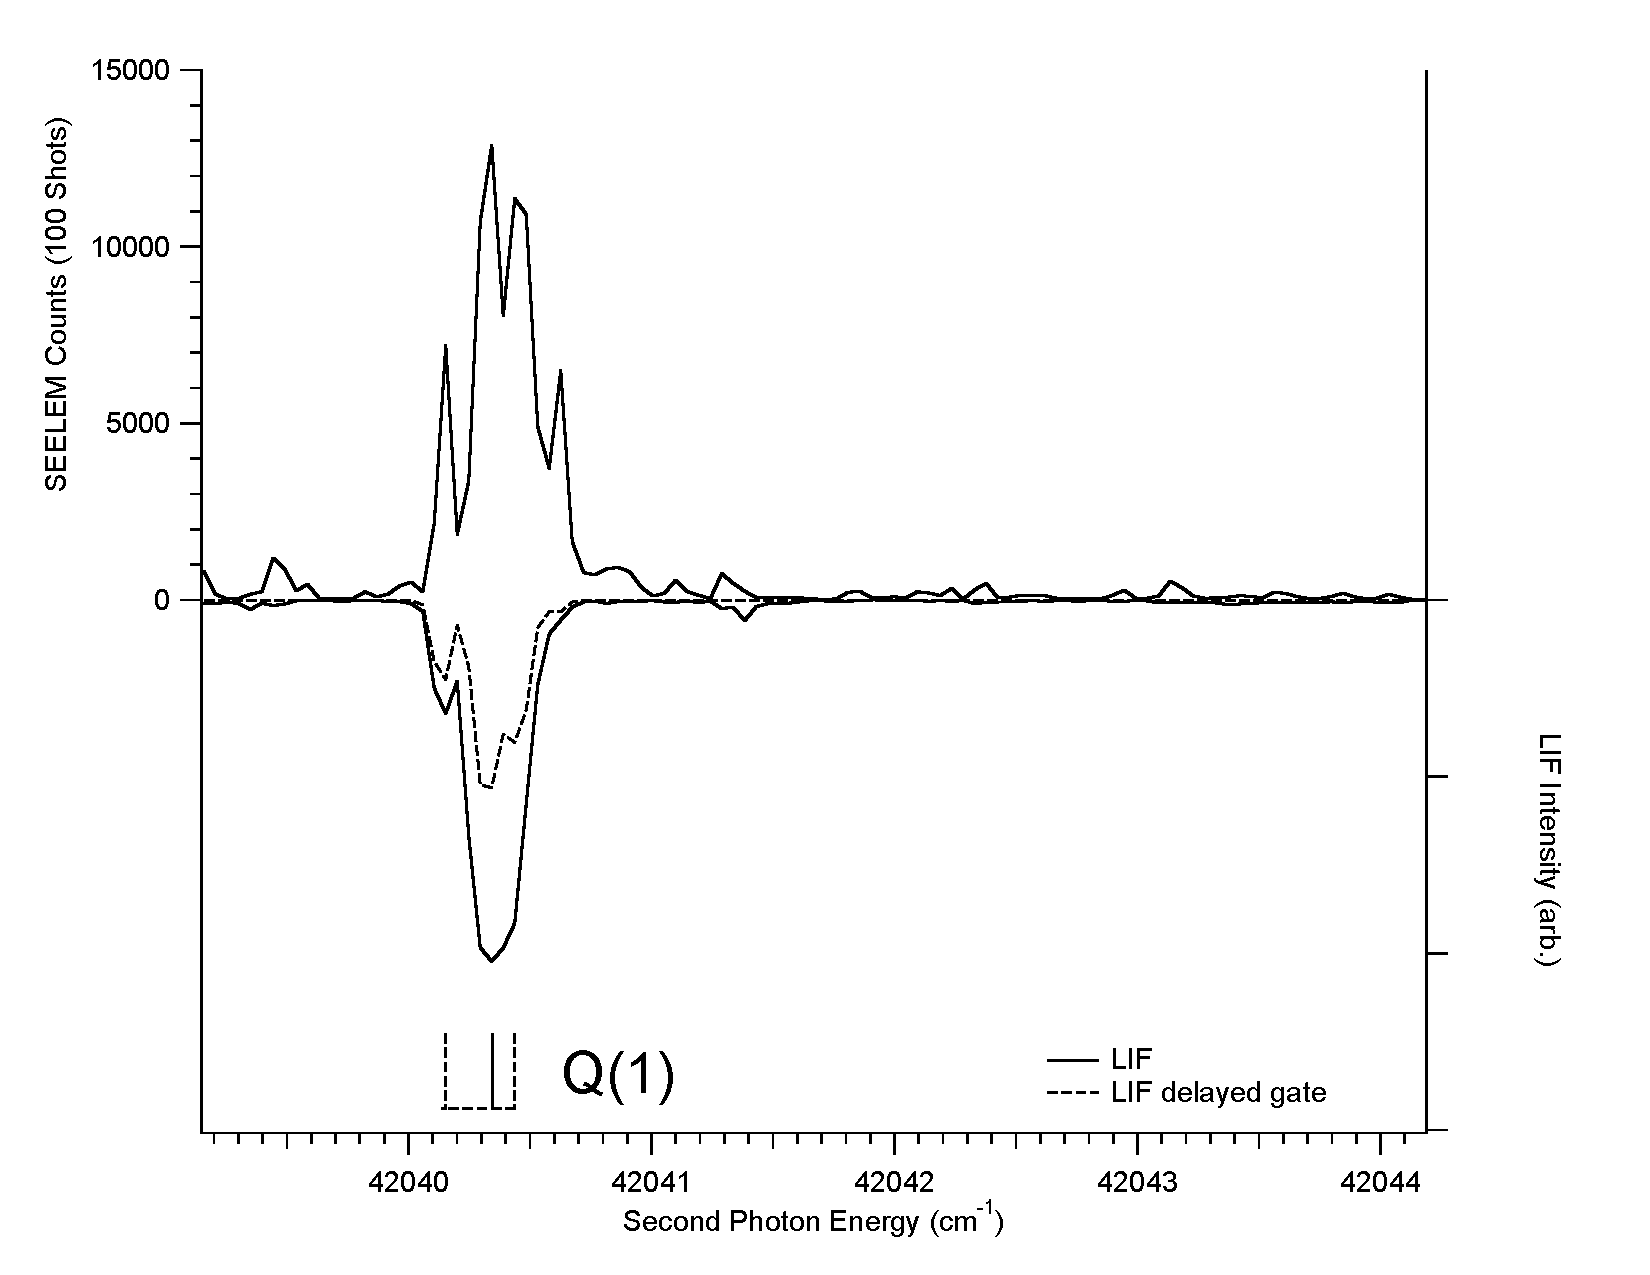
\includegraphics[width=6in]{spectrum-3361-q1-split.pdf}
  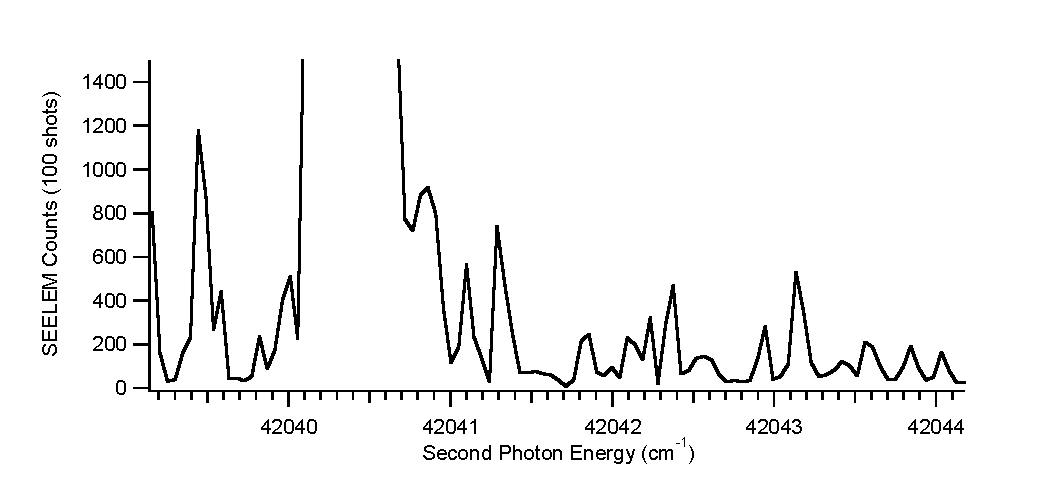
\includegraphics[width=5.5in]{spectrum-3361-q1-zoom.pdf}
\end{figure}

\begin{figure}
  \caption{Simultaneously recorded SEELEM (upper trace) and LIF (lower
    trace) spectra of the $3^36^1$ \Ka{0} sublevel of the \astate\
    state of \ce{C2H2}.  The P(3) line of the \xstate\ $\nu_3'' +
    \nu_4''$ level is used as an intermediate state in the experiment,
    so only the Q(2) line is observed in the upper state, according to
    Figure \ref{fig:levels-iruvdr}.  The LIF spectrum is integrated in
    two time regions: an early time window ($0.5\tau_s-2\tau_s$, solid
    trace) and a delayed time window ($10\tau_s-18\tau_s$, dashed
    trace).  A line splitting of $\sim 2$ \rcm\ is observed in the LIF
    spectrum, with the longer-lifetime (nominally triplet) component
    located at higher energy.}
  \label{fig:3361-q2}
  \centering
  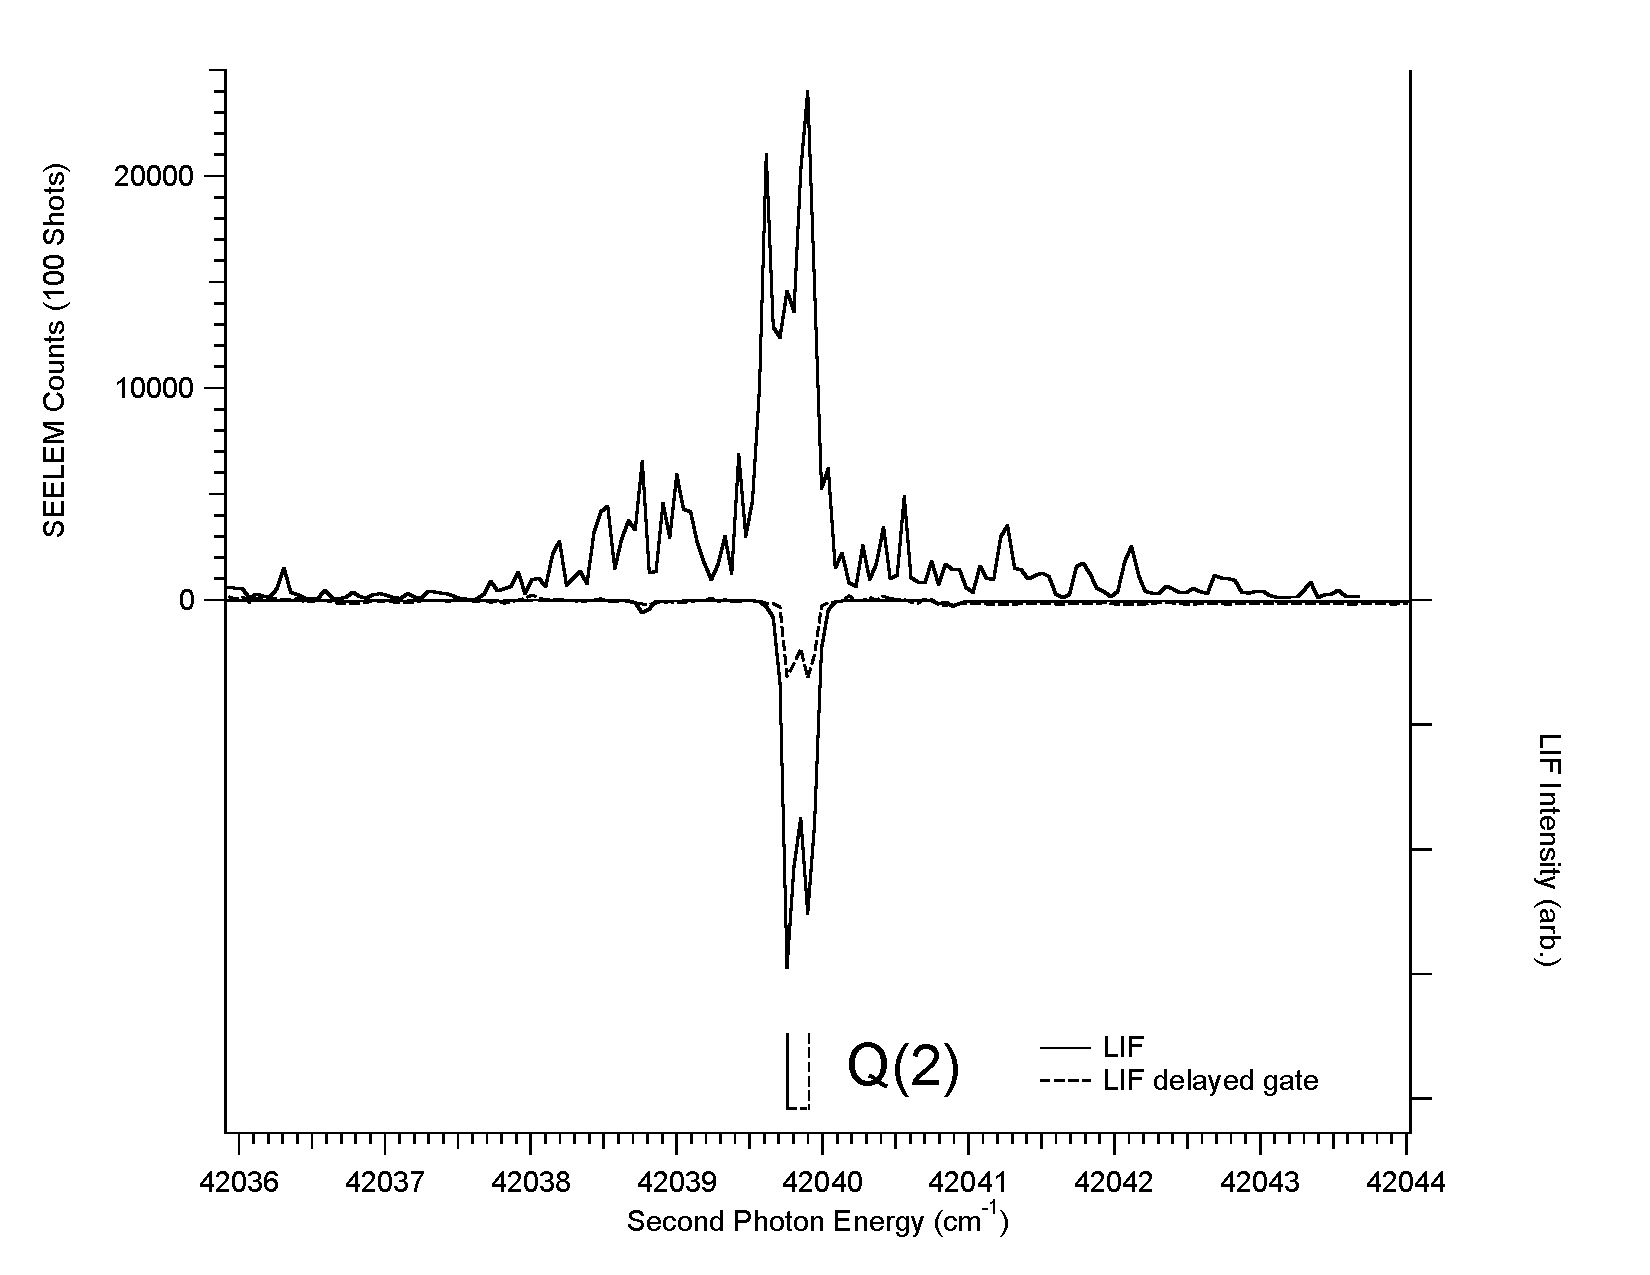
\includegraphics[width=6in]{spectrum-3361-q2-split.pdf}
  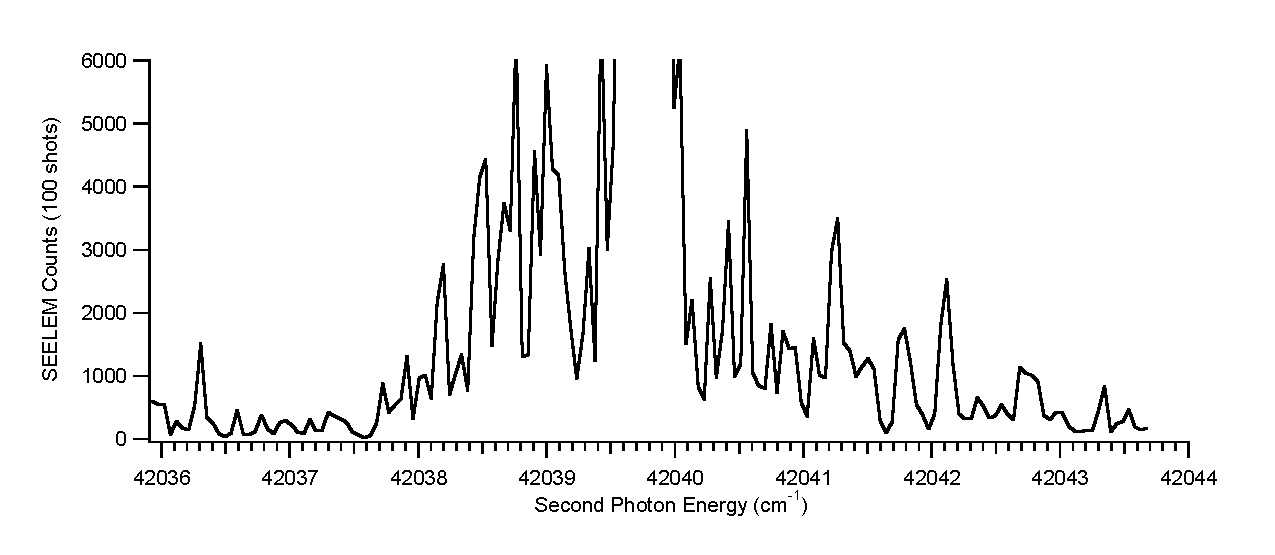
\includegraphics[width=6in]{spectrum-3361-q2-zoom.pdf}
\end{figure}

\begin{figure}
  \caption{Simultaneously recorded SEELEM (upper trace) and LIF (lower
    trace) spectra of the $3^36^1$ \Ka{0} sublevel of the \astate\
    state of \ce{C2H2}.  The P(4) line of the \xstate\ $\nu_3'' +
    \nu_4''$ level is used as an intermediate state in the experiment,
    so only the Q(3) line is observed in the upper state, according to
    Figure \ref{fig:levels-iruvdr}.  The LIF spectrum is integrated in
    two time regions: an early time window ($0.5\tau_s-2\tau_s$, solid
    trace) and a delayed time window ($10\tau_s-18\tau_s$, dashed
    trace).  The transition at 42038.3 \rcm\ has a short lifetime, and
    belongs to an unassigned singlet sublevel.  A small line splitting
    of less than $0.05$ \rcm\ is apparent from the shifted peak
    position in the delayed LIF spectrum relative to the early LIF
    spectrum.  The longer-lifetime (nominally triplet) component is
    located to higher energy.}
  \label{fig:3361-q3}
  \centering
  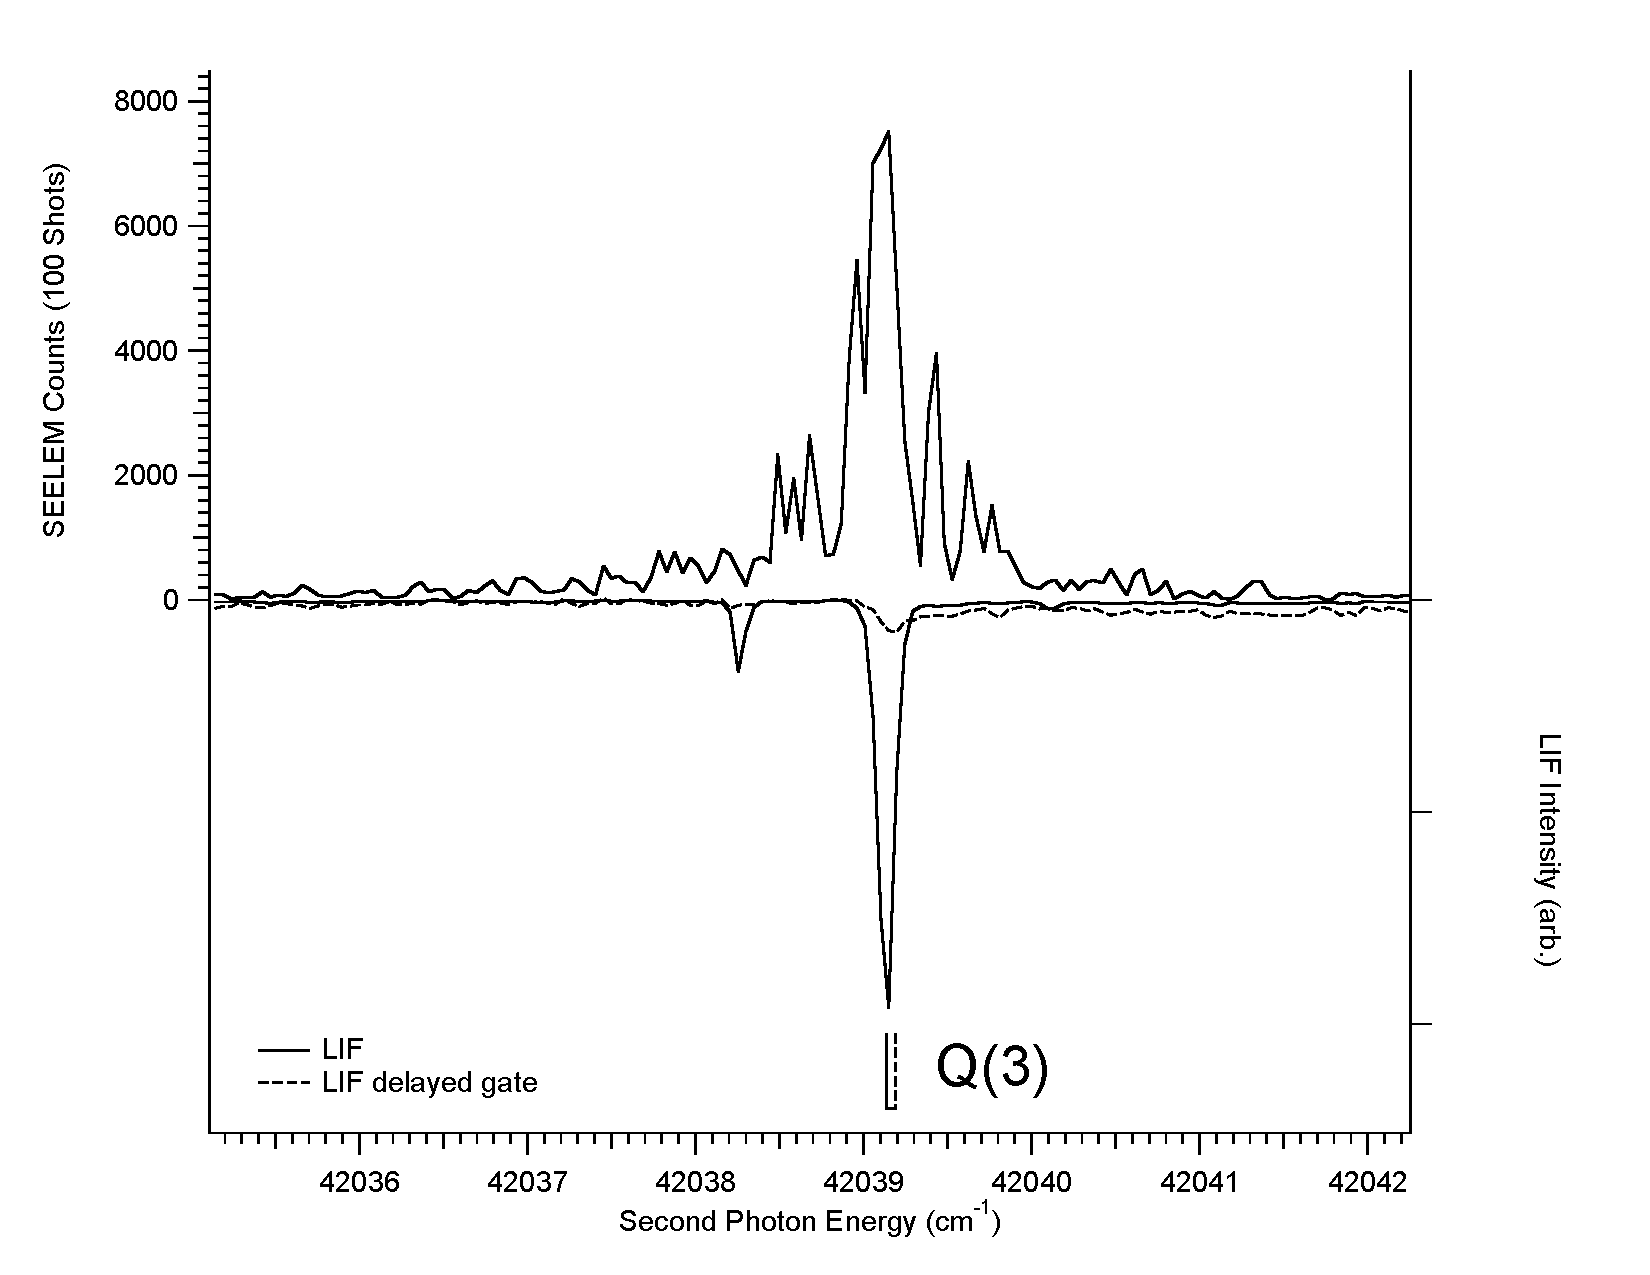
\includegraphics[width=6in]{spectrum-3361-q3-split.pdf}
  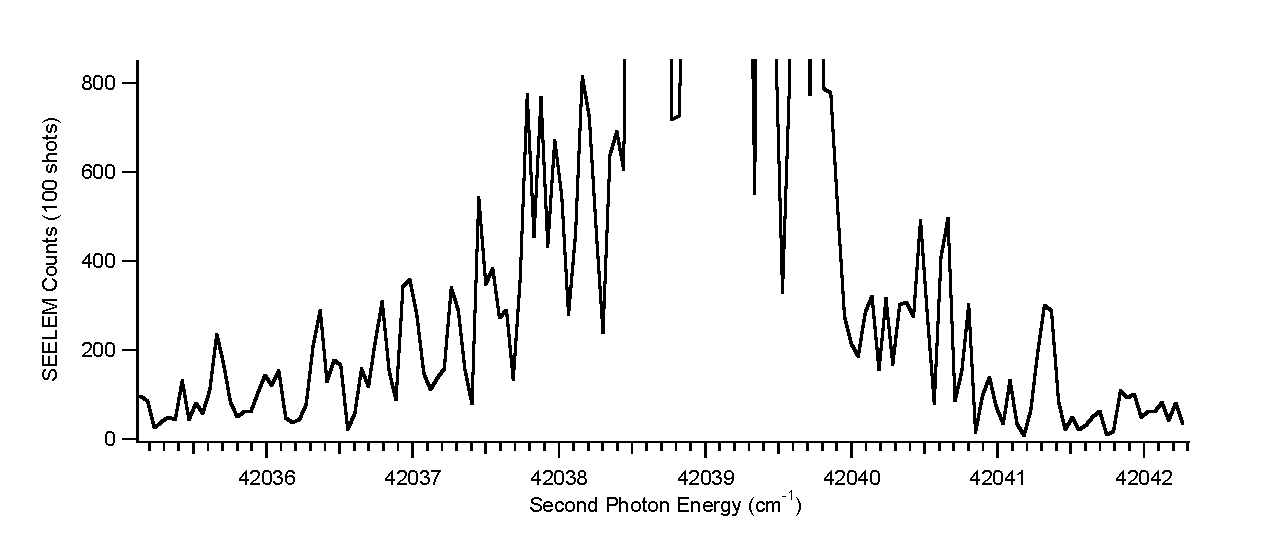
\includegraphics[width=6in]{spectrum-3361-q3-zoom.pdf}
\end{figure}

\begin{figure}
  \caption{Simultaneously recorded SEELEM (upper trace) and LIF (lower
    trace) spectra of the $3^36^1$ \Ka{0} sublevel of the \astate\
    state of \ce{C2H2}.  The R(3) line of the \xstate\ $\nu_3'' +
    \nu_4''$ level is used as an intermediate state in the experiment,
    so only the Q(4) line is observed in the upper state, according to
    Figure \ref{fig:levels-iruvdr}.  The LIF spectrum is integrated in
    two time regions: an early time window ($0.5\tau_s-2\tau_s$, solid
    trace) and a delayed time window ($10\tau_s-18\tau_s$, dashed
    trace).  A line splitting of $\sim0.2$ \rcm\ is observed in the LIF
    spectrum, with the longer-lifetime (nominally triplet) component
    located at higher energy.}
  \label{fig:3361-q4}
  \centering
  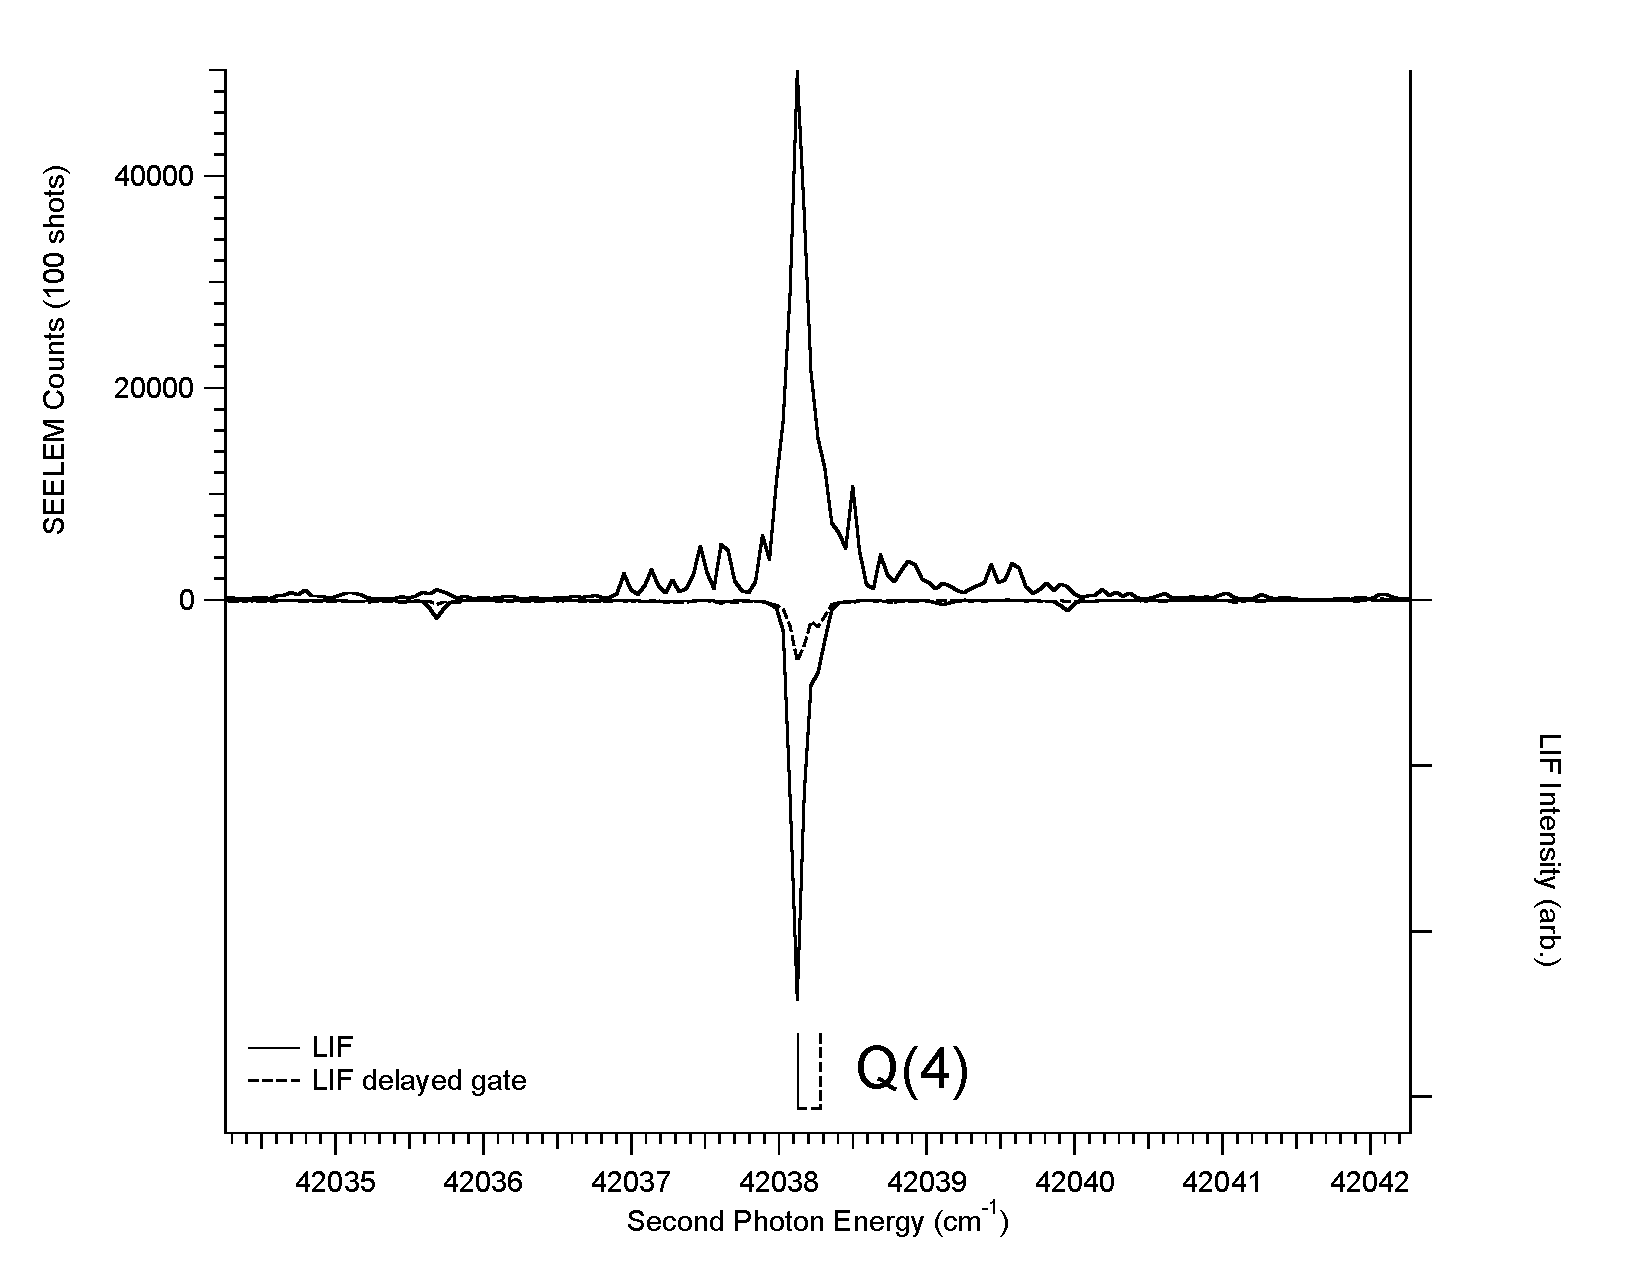
\includegraphics[width=6in]{spectrum-3361-q4-split.pdf}
  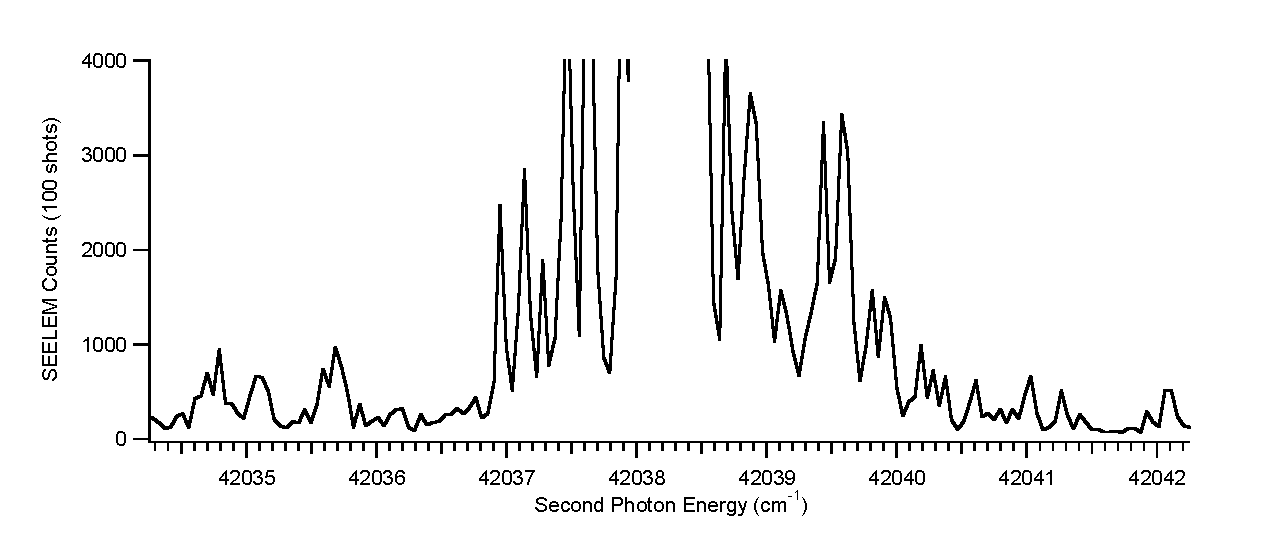
\includegraphics[width=6in]{spectrum-3361-q4-zoom.pdf}
\end{figure}

\begin{figure}
  \caption{Simultaneously recorded SEELEM (upper trace) and LIF (lower
    trace) spectra of the $3^36^1$ \Ka{0} sublevel of the \astate\
    state of \ce{C2H2}.  The R(4) line of the \xstate\ $\nu_3'' +
    \nu_4''$ level is used as an intermediate state in the experiment,
    so only the Q(5) line is observed in the upper state, according to
    Figure \ref{fig:levels-iruvdr}.  The LIF spectrum is integrated in
    two time regions: an early time window ($0.5\tau_s-2\tau_s$, solid
    trace) and a delayed time window ($10\tau_s-18\tau_s$, dashed
    trace).  No line splittings are observed in the LIF spectrum.}
  \label{fig:3361-q5}
  \centering
  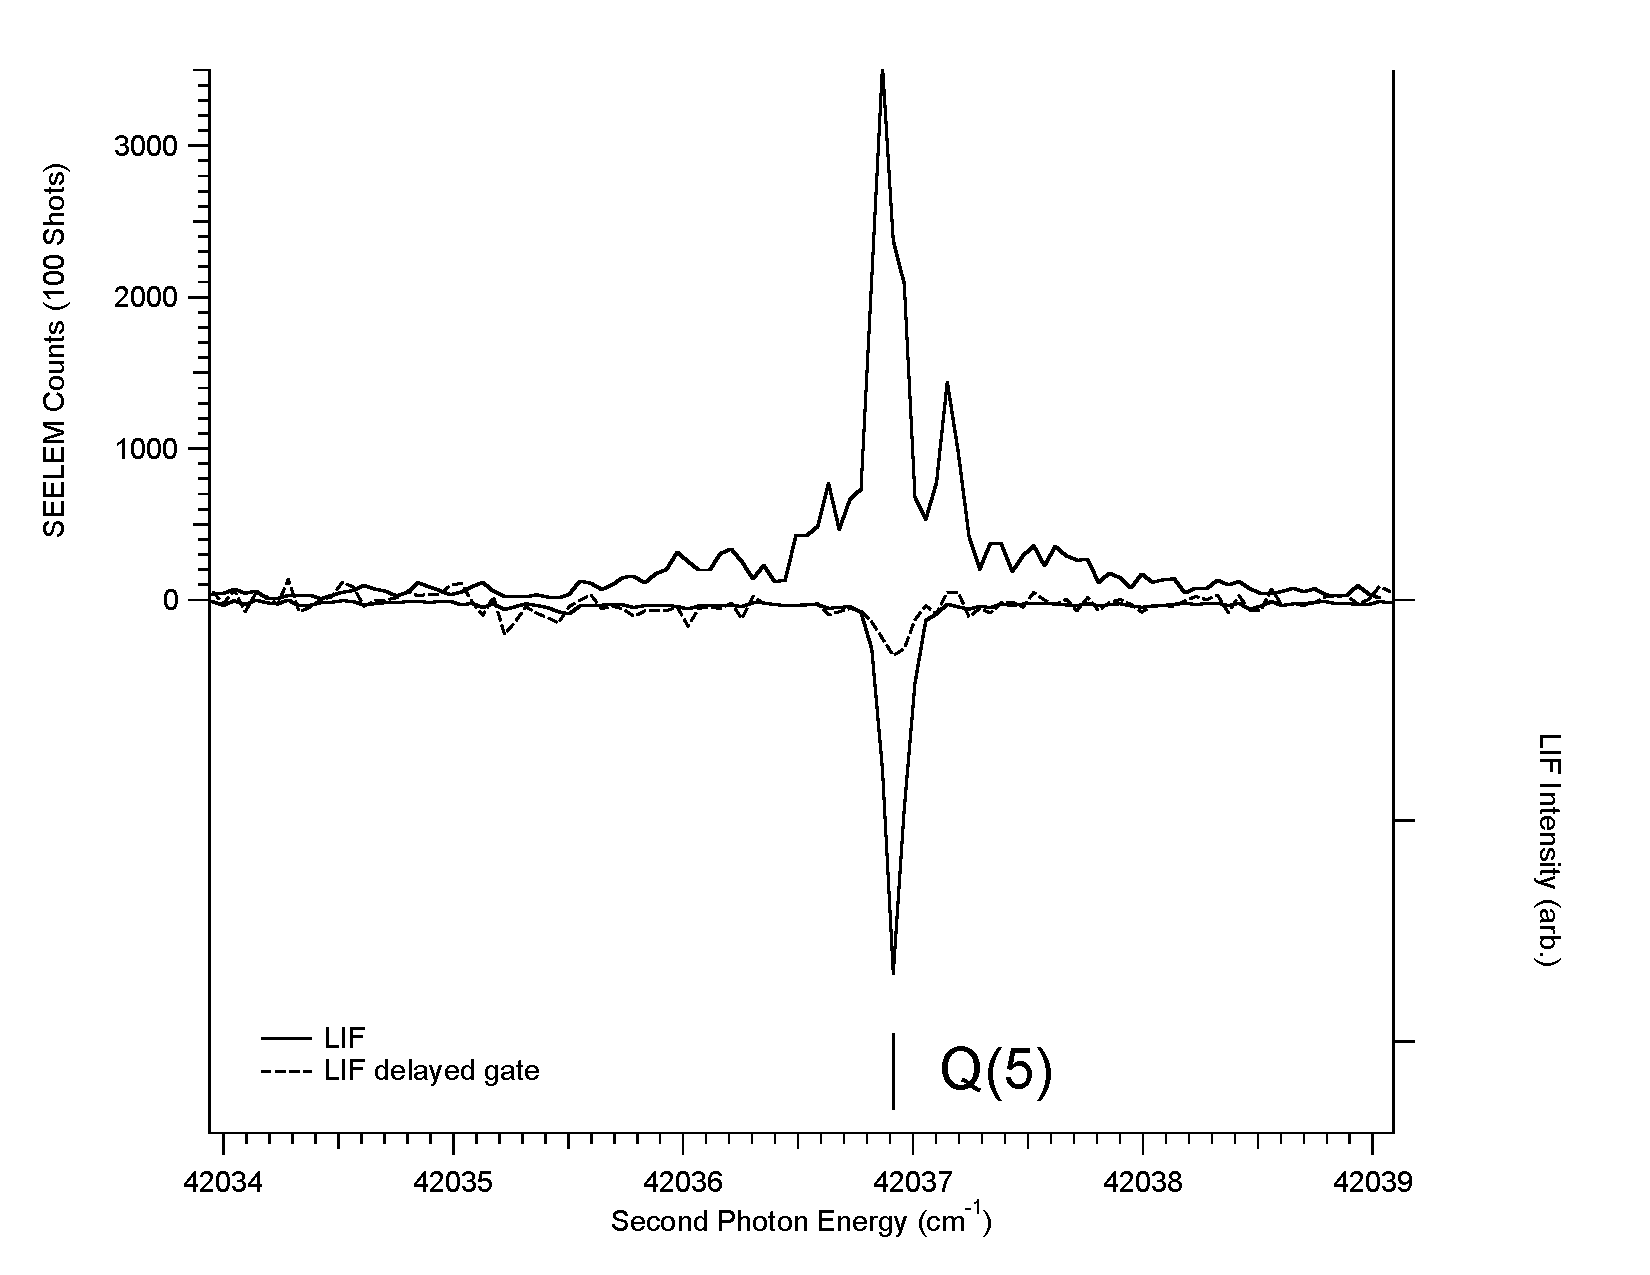
\includegraphics[width=6in]{spectrum-3361-q5-split.pdf}
  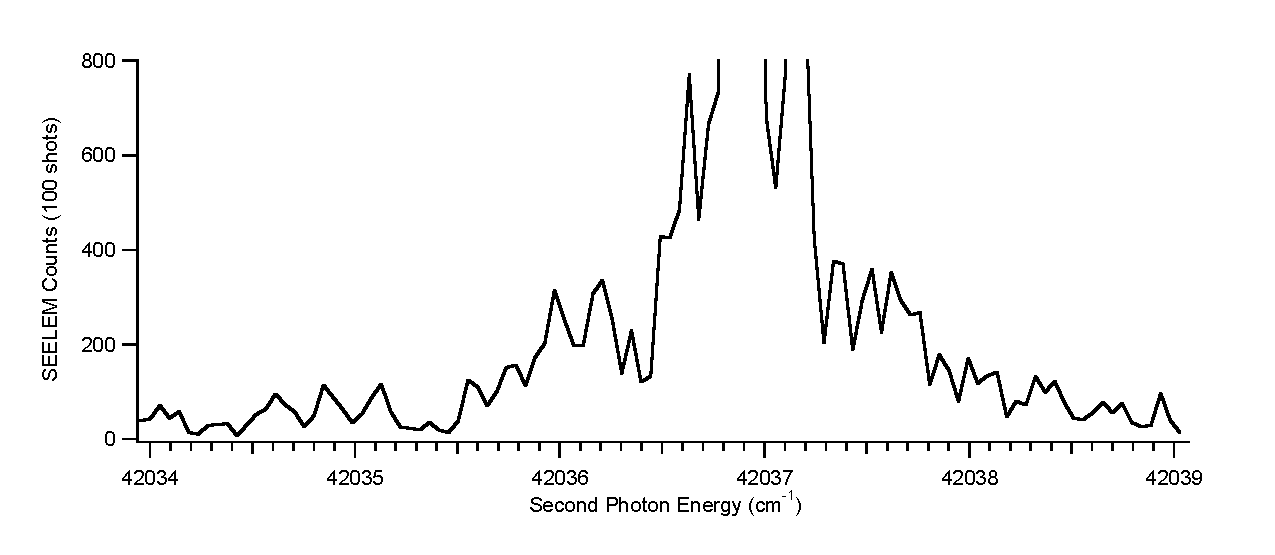
\includegraphics[width=6in]{spectrum-3361-q5-zoom.pdf}
\end{figure}

%%%%%%%%%%%%%%%%%%%%%%%%%%%%%%%%%%%%%%%%%%%%%%%%%%%%%%
%%
%% END OF 3^3 6^1 INDIV FIGURES
%%
%%%%%%%%%%%%%%%%%%%%%%%%%%%%%%%%%%%%%%%%%%%%%%%%%%%%%%

The spectrum of the $J'=0$ rotational level of $3^36^1$ \Ka{0} cannot
be recorded using the individual line double resonance method, since
the method permits only Q-branch transitions to appear in the UV
spectrum.  Instead, the spectrum of $3^36^1$ \Ka{0} $J'=0$ was
recorded in the region of the P(1) transition by the survey method,
using two relative polarization geometries for the IR and UV laser
beams.  When the polarization of the collinear IR and UV beams is
aligned in a perpedicular geometry, the P(1) transition, terminating
on $J''=0$, is permitted in the UV.  The two-step excitation proceeds
according to the following selection rules.  $M_J$ sublevels in the
intermediate state with $M_J=1$ are populated via $\Delta M_J=0$
transitions in the first excitation step.  In the second excitation
step, when the UV laser beam is perpedicularly polarized relative to
the IR beam, $\Delta M_J = \pm 1$ transitions are permitted to the
upper state $J'=0$ rotational level, which has only one $M_J$
component, $M_J=0$.  Figure \ref{fig:levels-polarization} illustrates
the permitted transitions among $M_J$ sublevels as solid arrows.

When the polarizations of the collinear IR and UV laser beams are
parallel, the selection rules for $\Delta M_J$ do not allow any
transitions that terminate in the upper state $J'=0$ rotational level.
Since the IR and UV beams have identical polarization, the value of
$\lvert \Delta M_J \rvert$ must be identical in the IR and UV
excitation steps.  A value of $\Delta M_J = + 1$ or $\Delta M_J = - 1$
in both steps does not accomodate transitions terminating in the
$J'=0$ rotational level of the excited state.  A value of $\Delta M_J
= 0$ for both steps could possibly terminate in the $J'=0$ rotational
level of the excited state, but such a transition is forbidden in the
first step, according to the selection rule that $M_J=0
\nleftrightarrow M_J=0$ for $\Delta J = 0$ (Q-branch) tansitions
\cite{herzberg66}.  The forbidden transition is illustrated with
dashed arrows in Figure \ref{fig:levels-polarization}.  According to
the selection rules for $\Delta M_J$, the transition to $J'=0$ in the
excited state is forbidden for parallel laser
polarization. \TODO{SPECIFY AXIS CONVENTION FOR EVALUATING Mj
  SELECTION RULES AND FOLLOW RIGOROUSLY. SUPPORT UNIVERSAL
  APPLICABILITY BY ASSERTING THAT WE ARE FREE TO CHOOSE THE LABORATORY
  AXIS SYSTEM.}

%%%%%%%%%%%%%%%%%%%%%%%%%%%%%%%%%%%%%%%%%%%%%%%%%%%%%%%
%%
%% INSERT POLARIZATION DIAGRAM
%%
%%%%%%%%%%%%%%%%%%%%%%%%%%%%%%%%%%%%%%%%%%%%%%%%%%%%%%%

\begin{figure}
  \caption{Diagram of transitions among hyperfine levels terminating
    in the $J'=0$ rotational level of $3^36^1$ \Ka{0}.  When the IR
    and UV lasers are polarized in a perpendicular geometry,
    transitions terminating in the $J'=0$ rotational level of the
    excited state are permitted according to the selection rules
    $\Delta M_J = 0$ (first step), $\Delta M_J = \pm 1$ (second step).
    When the IR and UV lasers are polarized in a parallel geometry,
    transitions terminating in the $J'=0$ rotational level of the
    excited state are forbidden according to the selection rule $M_J =
    0 \nleftrightarrow M_J = 0$ when $\Delta J = 0$.}
  \label{fig:levels-polarization}

  \centering
  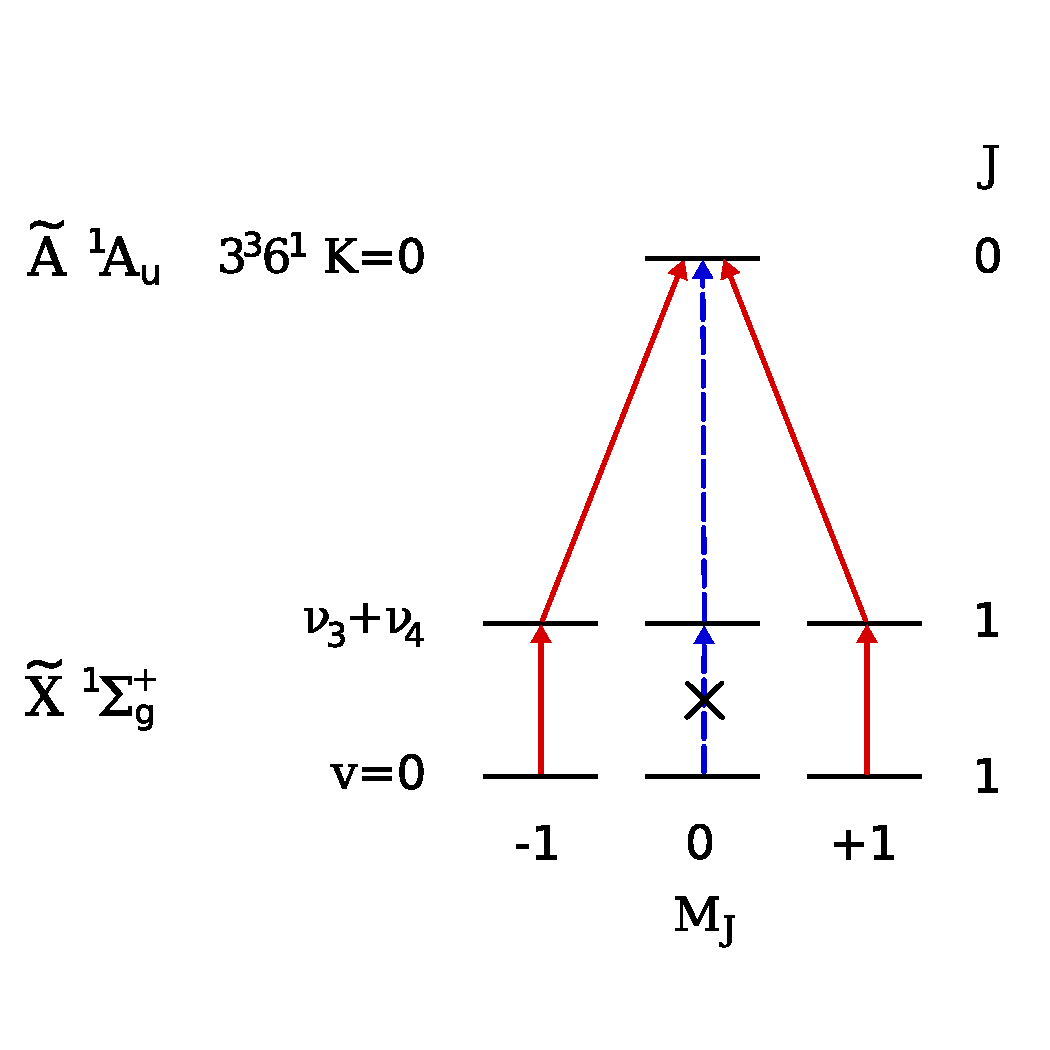
\includegraphics[width=5in]{levels-polarization.pdf}
\end{figure}

%%%%%%%%%%%%%%%%%%%%%%%%%%%%%%%%%%%%%%%%%%%%%%%%%%%%%%
%%
%% END POLARIZATION DIAGRAM
%%
%%%%%%%%%%%%%%%%%%%%%%%%%%%%%%%%%%%%%%%%%%%%%%%%%%%%%%

Simultaneously recorded SEELEM/LIF spectra in the region of the
$3^36^1$ \Ka{0} P(1) transition are shown in Figure
\ref{fig:3361-p1-polarization}, for perpendicular (solid trace) and
parallel (dashed trace) laser polarization.  Since the transition to
$J'=0$ is forbidden in the parallel geometry, the dashed trace serves
as a null spectrum in this region.  At UV frequencies between 42036.0
and 42041.3 \rcm, essentially all peaks in the SEELEM spectrum are due
to intensity borrowing from the $J'=0$ level of $3^36^1$ \Ka{0}.  This
particular region is shown with more detail in Figure
\ref{fig:3361-p1}.  The delayed LIF spectrum is also included as a
dashed trace in this figure.  A line splitting is resolved in the
delayed LIF spectrum, with the long-lifetime component lying to higher
frequency.

%%%%%%%%%%%%%%%%%%%%%%%%%%%%%%%%%%%%%%%%%%%%%%%%%%%%%%
%%
%% INSERT 3^3 6^1 POLARIZATION FIGURES HERE
%%
%%%%%%%%%%%%%%%%%%%%%%%%%%%%%%%%%%%%%%%%%%%%%%%%%%%%%%

\begin{figure}
  \caption{Simultaneously recorded SEELEM (upper trace) and LIF (lower
    trace) spectra of the $3^36^1$ \Ka{0} sublevel of the \astate\
    state of \ce{C2H2}.  The Q-branch of the \xstate\ $\nu_3'' +
    \nu_4''$ level is used as an intermediate transition in the
    experiment.  As a result, P- and R-branch lines are observed in
    the upper state, according to Figure \ref{fig:levels-iruvdr}.  The
    P(1) transition to the upper state is forbidden in a parallel
    IR-UV laser polarization geometry.  A spectrum recorded with this
    laser geometry is shown as a dashed line. \TODO{Label SEELEM peaks
      in P(1)}}
  \label{fig:3361-p1-polarization}
  \centering
  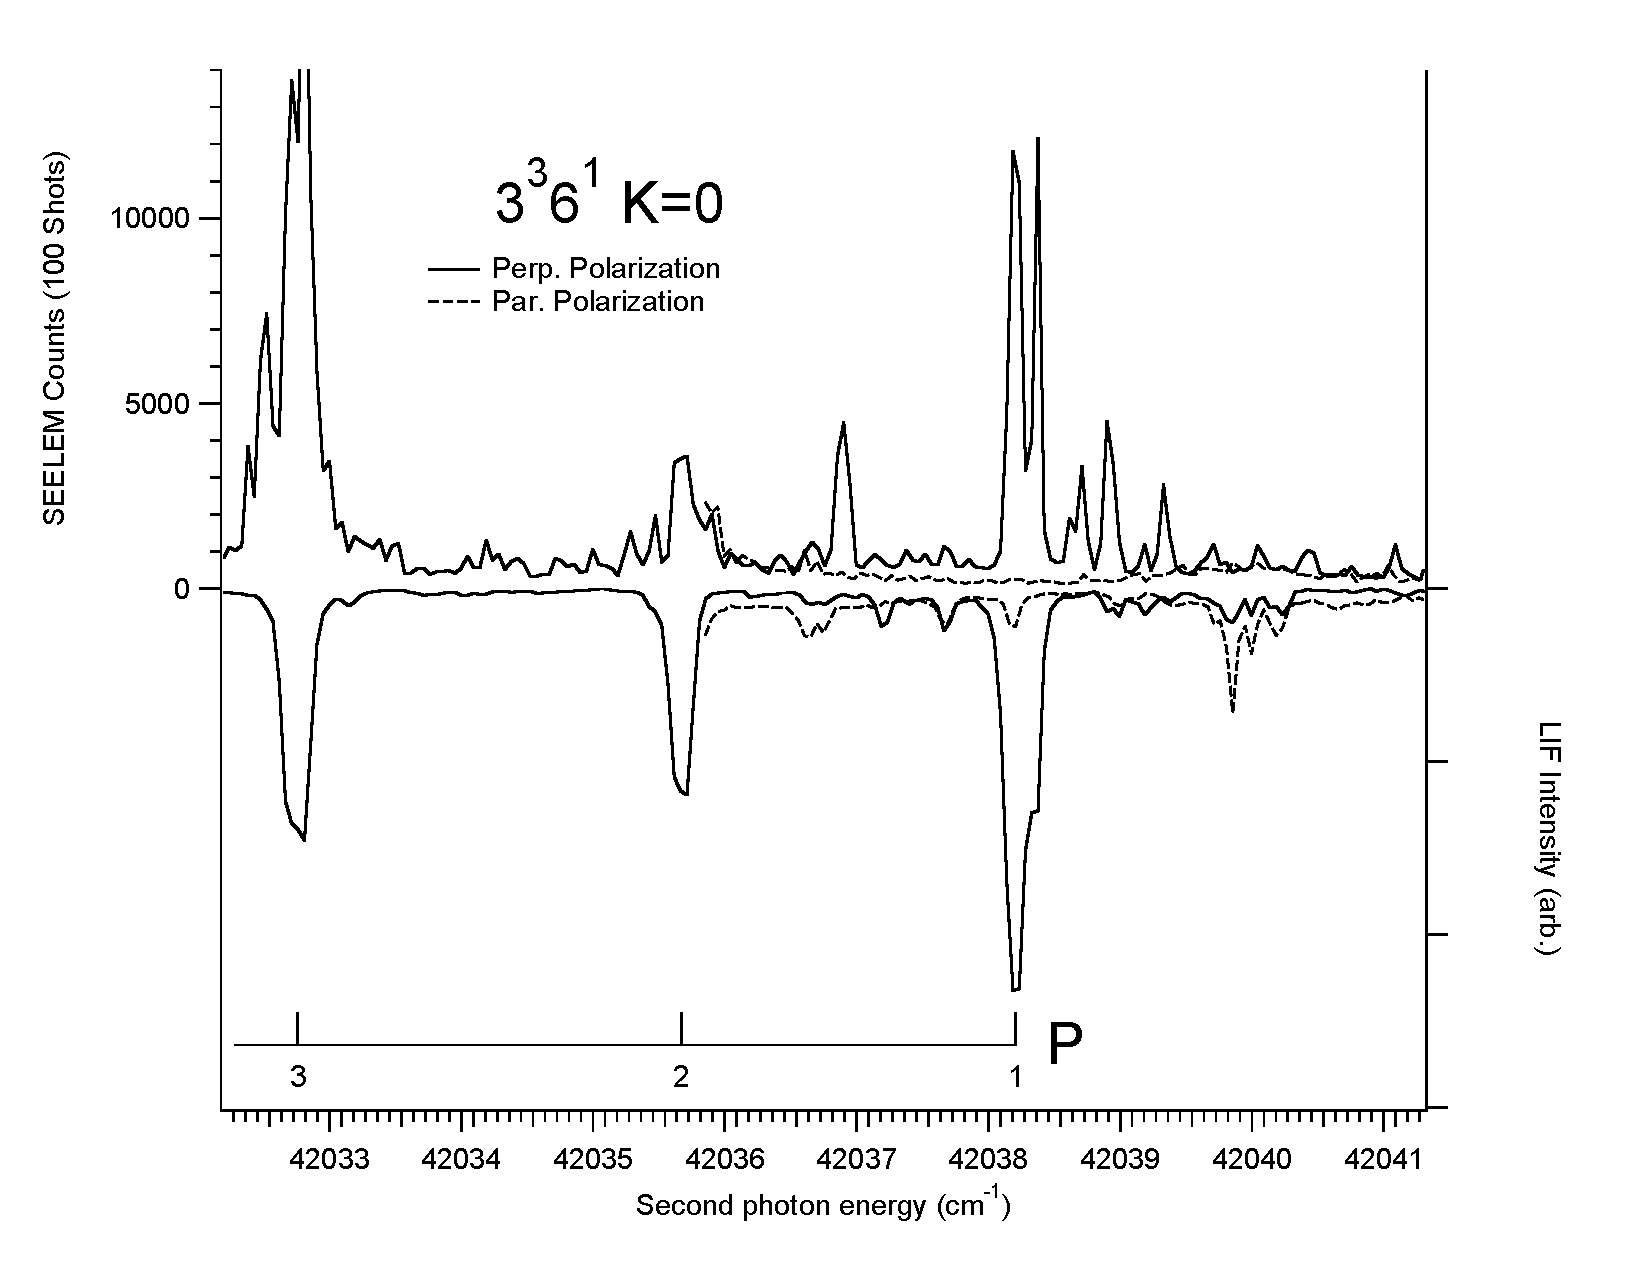
\includegraphics[width=7.3in,angle=90]{spectrum-3361-p1.pdf}
\end{figure}


\begin{figure}
  \caption{Simultaneously recorded SEELEM (upper trace) and LIF (lower
    trace) spectra of the $3^36^1$ \Ka{0} sublevel of the \astate\
    state of \ce{C2H2}.  The Q-branch of the \xstate\ $\nu_3'' +
    \nu_4''$ level is used as an intermediate transition in the
    experiment.  As a result, P- and R-branch lines are observed in
    the upper state, according to Figure \ref{fig:levels-iruvdr}.  The
    LIF spectrum is integrated in two time regions: an early time
    window ($0.5\tau_s-2\tau_s$, solid trace) and a delayed time
    window ($10\tau_s-18\tau_s$, dashed trace).  A line splitting of
    $\sim 2$ \rcm\ is observed in the LIF spectrum, with the
    longer-lifetime (nominally triplet) component located at higher
    energy.}
  \label{fig:3361-p1}
  \centering
  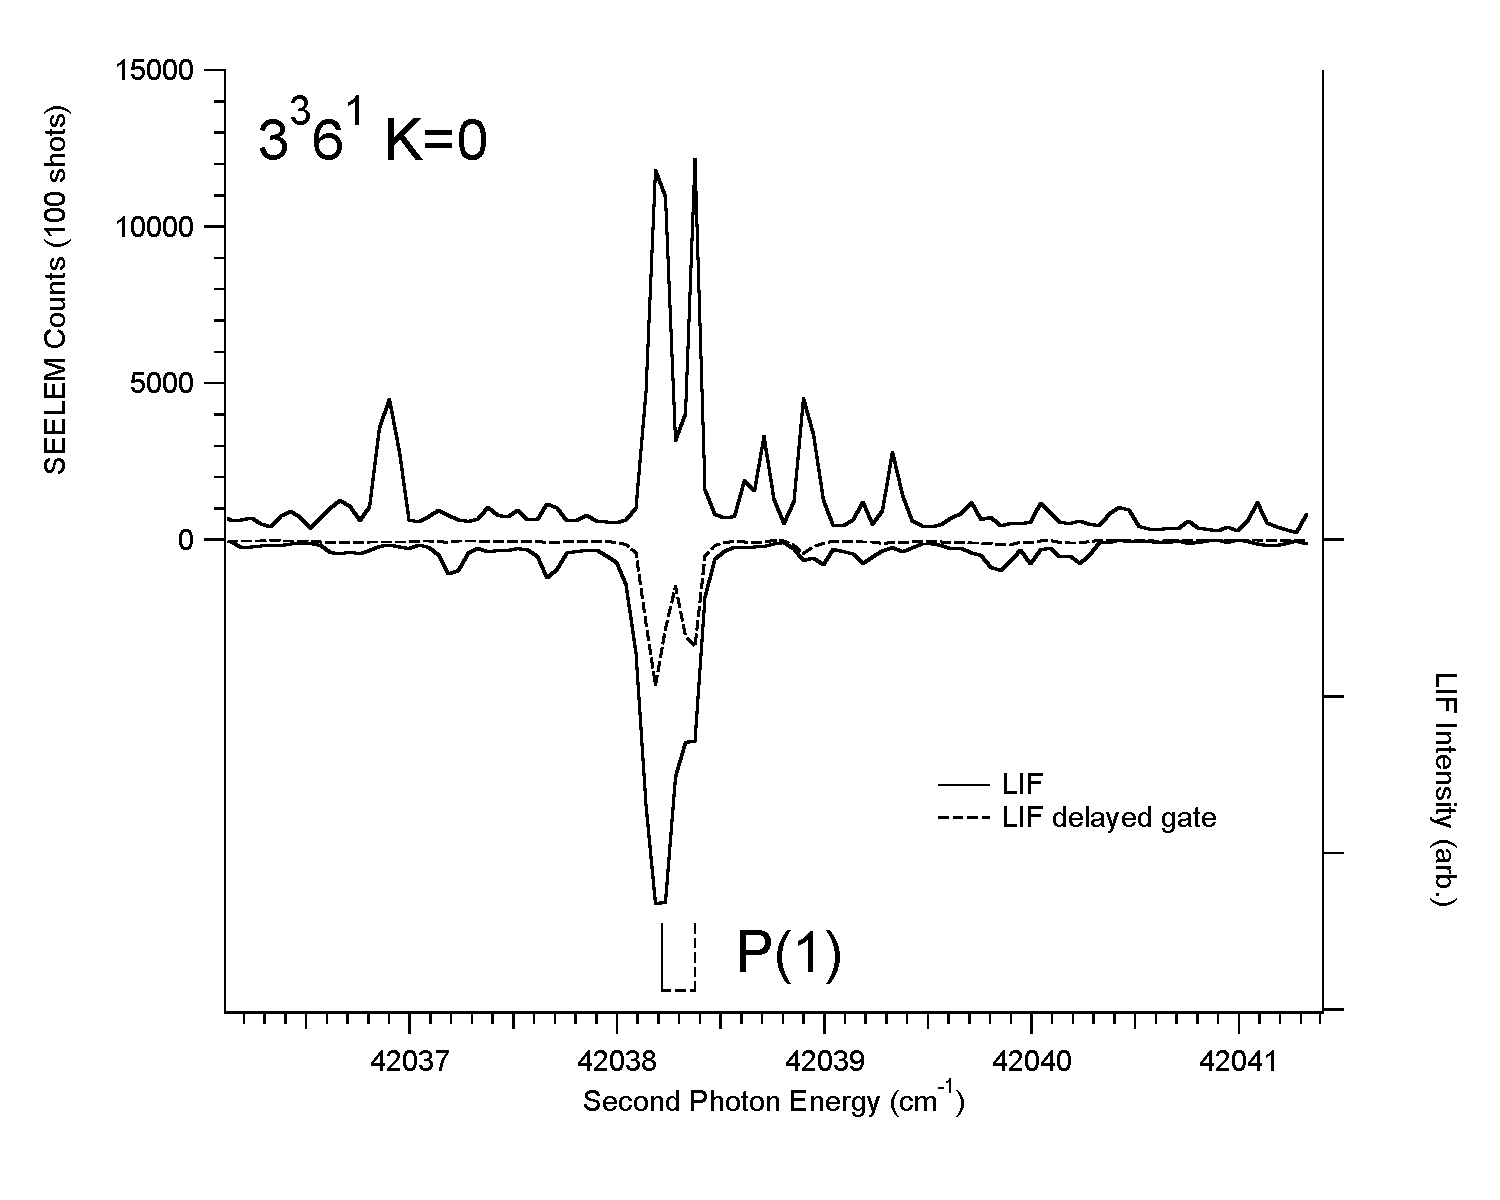
\includegraphics[width=5.8in]{spectrum-3361-p1-split}
  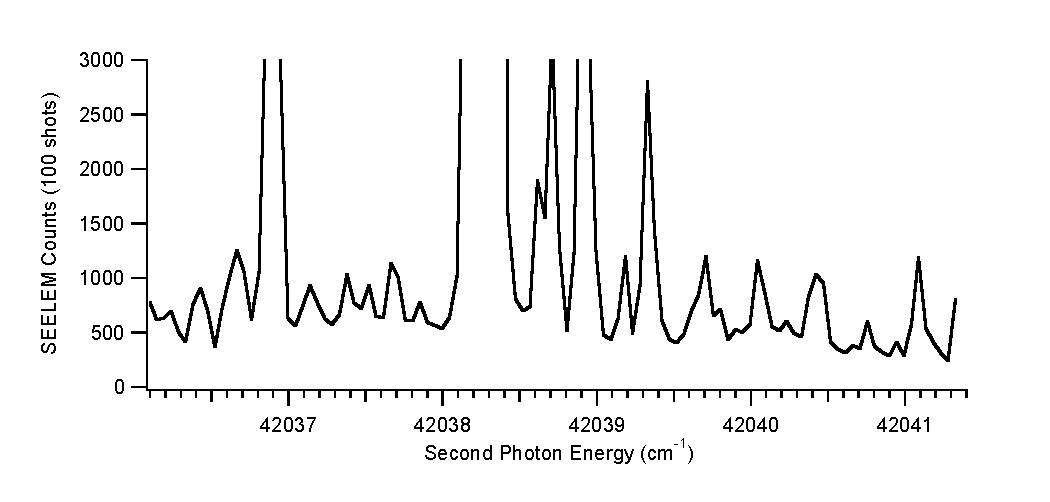
\includegraphics[width=6in]{spectrum-3361-p1-zoom}
\end{figure}

%%%%%%%%%%%%%%%%%%%%%%%%%%%%%%%%%%%%%%%%%%%%%%%%%%%%%%
%%
%% END OF 3^3 6^1 POLARIZATION FIGURES
%%
%%%%%%%%%%%%%%%%%%%%%%%%%%%%%%%%%%%%%%%%%%%%%%%%%%%%%%

The SEELEM/LIF spectrum of $3^34^1$ \Ka{0}, recorded by the survey
method, is shown in Figure \ref{fig:survey-3341}.  The LIF spectrum is
integrated in both early ($0.5\tau_s-2\tau_s$, solid trace) and
delayed ($10\tau_s-18\tau_s$, dashed trace) time windows.  Due to
saturation of the photomultiplier tube at early time intervals, the
early LIF spectrum shown in the figure was recorded and calibrated in
a separate scan.  The delayed LIF spectrum and the SEELEM spectrum
were acquired simultaneously.  The integrated SEELEM:LIF intensity
ratio is observed to be on the same order of magnitude as that of the
$3^36^1$ \Ka{0} level.

Line splittings appear in the delayed LIF spectrum of every transition
to the $3^34^1$ \Ka{0} sublevel.  The splittings span a frequency
range of $0.06-0.3$ \rcm.  The average frequency difference between
components having the same $J'$ is slightly larger than that of
$3^36^1$ \Ka{0}, and in general the splittings are more pronounced in the early
LIF spectrum.  Presumably the line splittings in $3^34^1$ \Ka{0} were
too small to be detected by Mizoguchi and coworkers, who recorded and
assigned the LIF spectrum of this level previously, and cite a UV
laser resolution of 0.1 \rcm \cite{mizoguchi00}.  Line splittings
reported in that reference, observed in another sublevel, are an order
of magnitude larger than those observed in this spectrum.

The line splitting in Q(1) could not be assigned directly from the
survey spectrum, because the long-lifetime component appears at a
frequency halfway between the Q(1) and Q(2) transitions.  To assign
the long-lifetime component, the spectrum of the P(2) transition in
$3^34^1$ \Ka{0} was recorded using the individual line method, via the P(3)
transition from the ground state.  This spectrum is shown in Figure
\ref{fig:3341-p2}.  A large line splitting of -0.25 \rcm\ is observed
in the LIF spectrum, confirming the assignment of the long-lifetime
component in Q(1) (Figure \ref{fig:survey-3341}).

%%%%%%%%%%%%%%%%%%%%%%%%%%%%%%%%%%%%%%%%%%%%%%%%%%%%%%
%%
%% INSERT 3^3 4^1 FIGURES HERE
%%
%%%%%%%%%%%%%%%%%%%%%%%%%%%%%%%%%%%%%%%%%%%%%%%%%%%%%%

\begin{figure}
  \caption{Simultaneously recorded SEELEM (upper trace) and LIF (lower
    trace) spectra of the $3^34^1$ \Ka{0} sublevel of the \astate\
    state of \ce{C2H2}.  The Q-branch of the \xstate\ $\nu_3'' +
    \nu_4''$ level is used as an intermediate transition in the
    experiment.  As a result, Q-branch lines are observed in the upper
    state, according to Figure \ref{fig:levels-iruvdr}.  The LIF
    spectrum is integrated in two time regions: an early time window
    ($0.5\tau_s-2\tau_s$, solid trace) and a delayed time window
    ($10\tau_s-18\tau_s$, dashed trace).  Line splittings ranging from
    0.06 to 0.3 \rcm\ are observed in the delayed LIF spectrum of all
    rotational lines.  With one exception, the longer-lifetime
    (nominally triplet) components are located at lower energy than
    the shortest-lifetime (nominally singlet) component. \TODO{prime K in figure}}
  \label{fig:survey-3341}
  \centering
  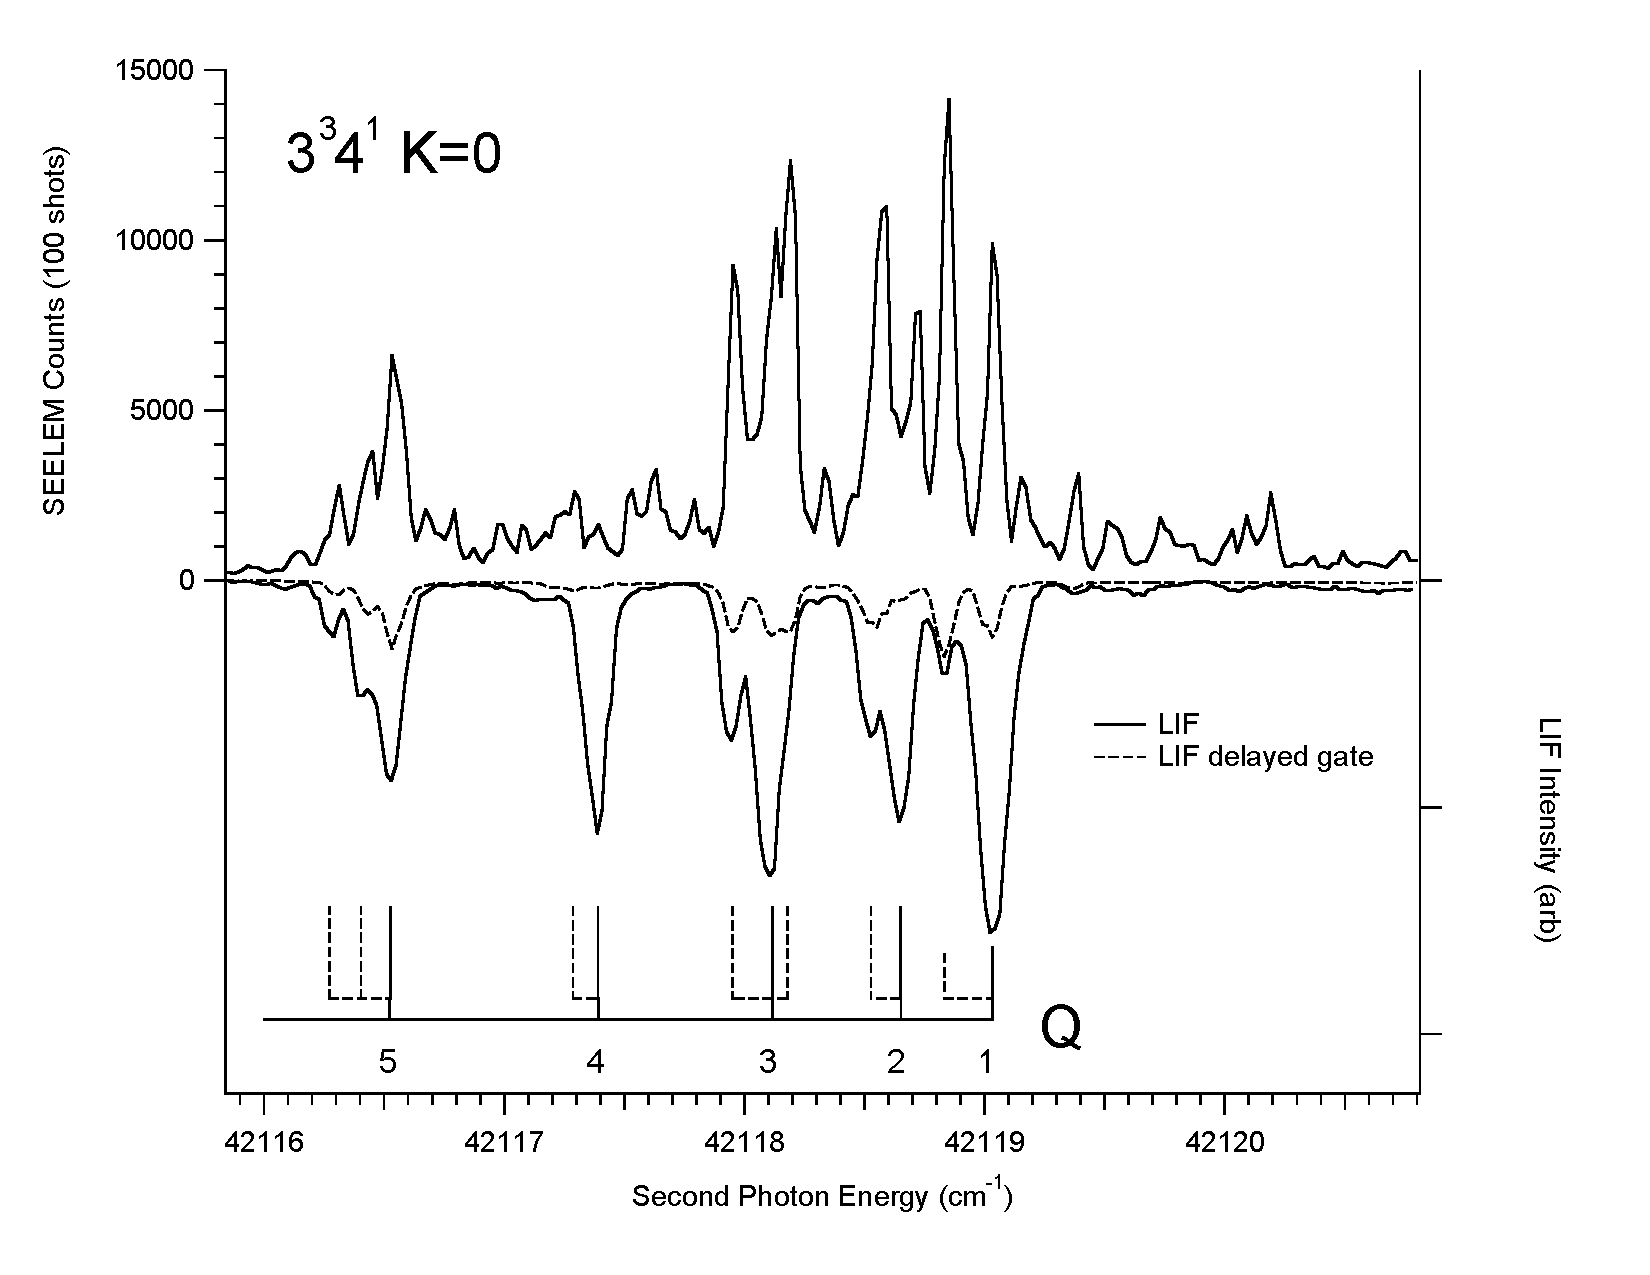
\includegraphics[width=7in,angle=90]{spectrum-3341-q5q1-split.pdf}
\end{figure}

\begin{figure}
  \caption{Simultaneously recorded SEELEM (upper trace) and LIF (lower
    trace) spectra of the $3^34^1$ \Ka{0} sublevel of the \astate\
    state of \ce{C2H2}.  The P(3) line of the \xstate\ $\nu_3'' +
    \nu_4''$ level is used as an intermediate state in the experiment,
    so only the P(2) line is observed in the upper state, according to
    Figure \ref{fig:levels-iruvdr}.  The LIF spectrum is integrated in
    two time regions: an early time window ($0.5\tau_s-2\tau_s$, solid
    trace) and a delayed time window ($10\tau_s-18\tau_s$, dashed
    trace).  A large line splitting of -0.25 \rcm\ is observed in the
    delayed fluorescence, confirming the assignment of the low-energy
    component as $J'=1$.  \TODO{Calibration, prime K in figure.}}
  \label{fig:3341-p2}
  \centering
  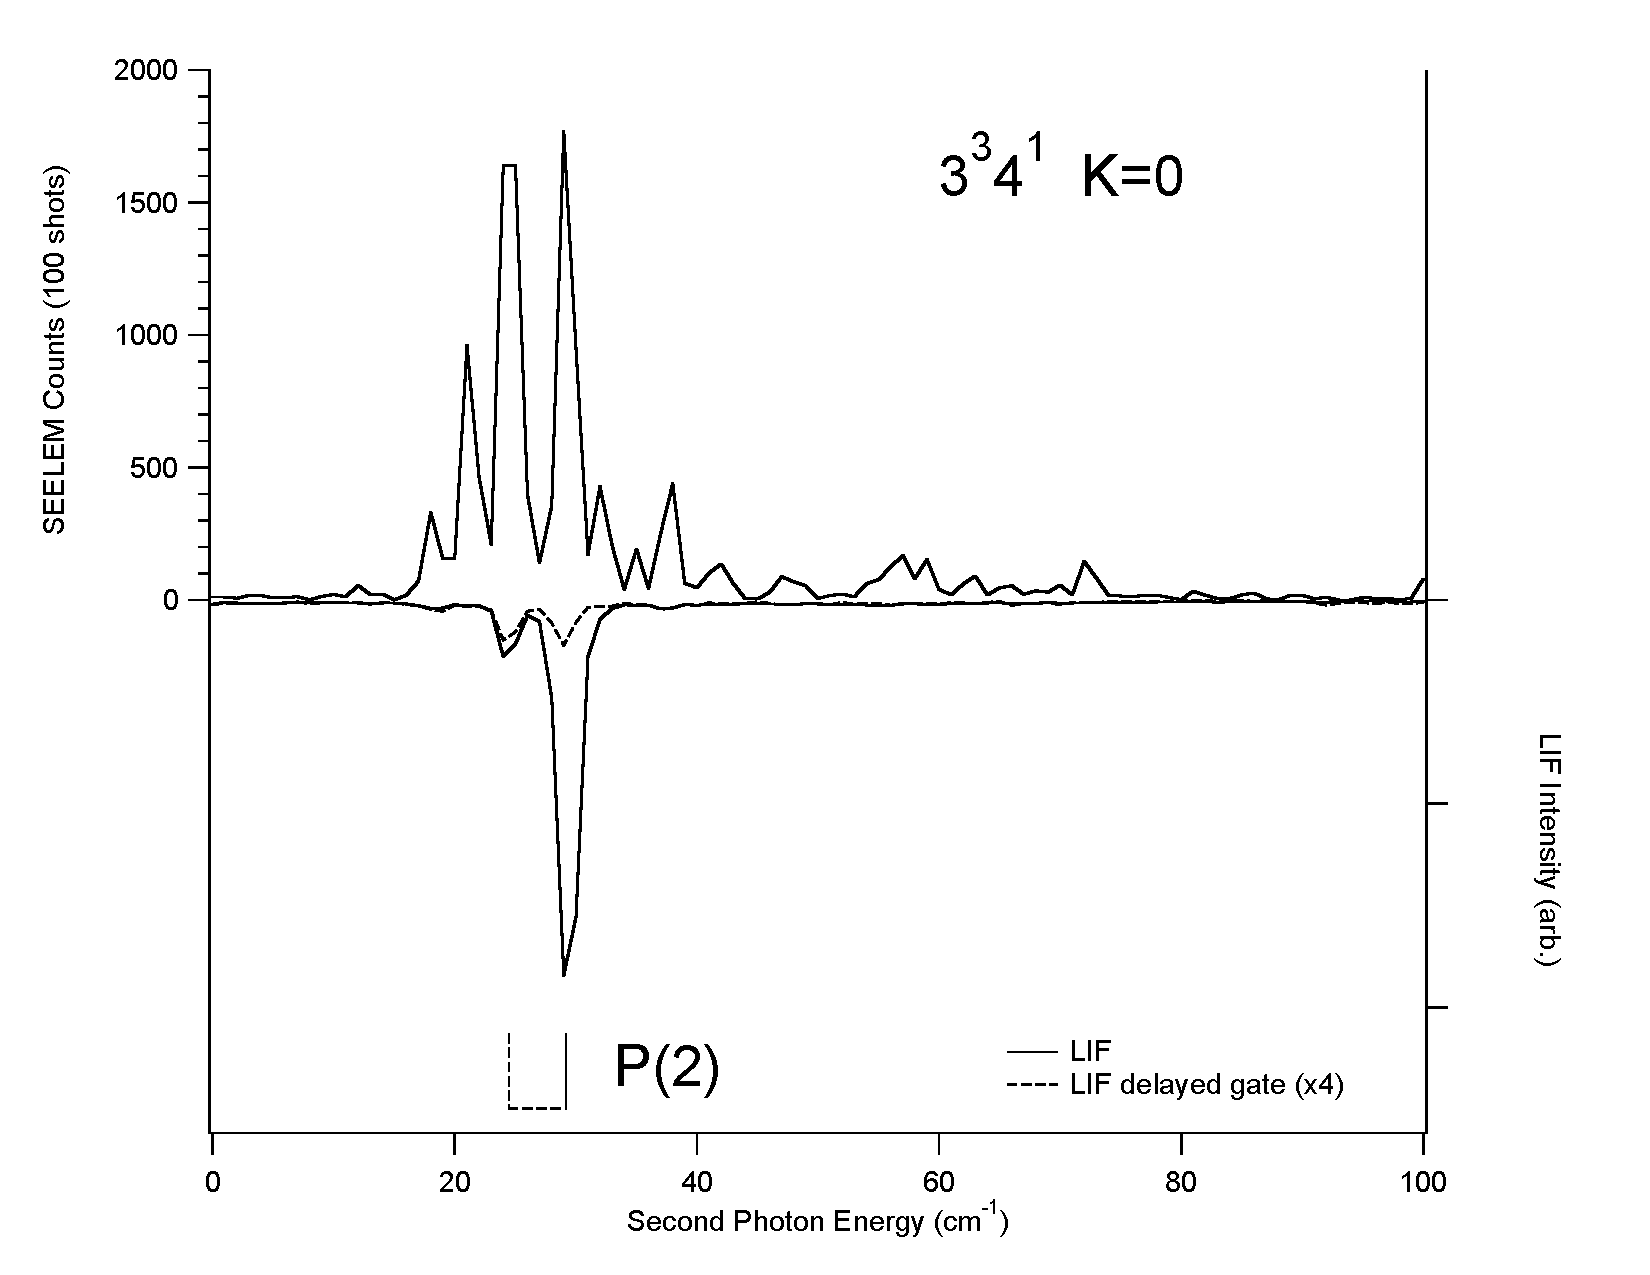
\includegraphics[width=6in]{spectrum-3341-p2-split.pdf}
\end{figure}

%%%%%%%%%%%%%%%%%%%%%%%%%%%%%%%%%%%%%%%%%%%%%%%%%%%%%%
%%
%% END OF 3^3 4^1 FIGURES
%%
%%%%%%%%%%%%%%%%%%%%%%%%%%%%%%%%%%%%%%%%%%%%%%%%%%%%%%













































\section{Analysis}

\subsection{LIF Spectrum: \\Characterization of mediating $T_3$
  levels}

Line splittings on the order of $0.2$ \rcm\ were observed in the LIF
spectrum of both $S_1$ sublevels, $3^36^1$ \Ka{0} and $3^34^1$ \Ka{0}.
Because the extra lines appear with greater intensity in the delayed
LIF spectrum relative to the early LIF spectrum, they are attributed
to mixing between the $S_1$ sublevel and nearby triplet levels.  Three
triplet electronic states are energetically accessible: $T_1$, $T_2$,
and $T_3$.  According to the doorway model for acetylene, mixing
between $S_1$ levels and the local manifold of $T_{1,2}$ triplet
levels is mediated by specific vibrational levels of the $T_3$
electronic state \TODO{cite}.  The vibrational levels of $T_3$ are
widely spaced, having an average level spacing on the order of 10 \rcm
\cite{thom07}.  In the majority of cases, the $T_3$ levels, which
mediate $S_1 \sim T_{1,2}$ mixing, do not appear in the spectrum of an
$S_1$ transition.  However, the spectrum contains evidence of the
presence of remote $T_3$ doorway levels, primarily as a result of the
$J'$-dependence of $S_1 \sim T_3$ energy denominators.  Four examples
of this behavior were discussed in Chapter 4. \TODO{Define local,
  remote.}

An analysis of the early vs. delayed LIF spectrum is our primary tool
for characterizing such non-local doorway states.  In Chapter 4.3, it was
shown that a non-local $T_3$ doorway level gives rise to a shift in
the LIF center of gravity,
\begin{equation}
  E_{\text{ave}} = \int E \times I(E) \; dE,
\end{equation}
when studied as a function of time delay.  The effect results from
drastically shorter fluorescence lifetime for the nominal $S_1$
eigenstate relative to nearby, nominally triplet eigenstates.  The
contrast in fluorescence liftimes leads to changes in relative
eigenstate intensity as a function of time: at early times, the center
of gravity is dominated by the nominal $S_1$ state, while at longer
delay times, the center of gravity is dominated by nominally triplet
eigenstates.  However, if the nominal $S_1$ eigenstate acquires more
triplet character, the contrast in fluorescence lifetimes is reduced,
deceasing the rate of change in center of gravity vs. time delay.

The relatively large line splittings observed in the spectrum of
$3^36^1$ \Ka{0} and $3^34^1$ \Ka{0} levels indicate that nominal $S_1$
eigenstates in these levels are appreciably singlet-triplet mixed.  To
make matters more complicated, the LIF spectra in this experiment
suffer from some saturation of the fluorescence signal at early time
delays, when the relative fluorescence intensity of the nominal $S_1$
state is at a maximum. We are thus precluded from using the center of
gravity vs. time as a diagnostic of the relative $T_3$ doorway energy,
as we were able to do with the spectrum of $3^3$ \Ka{2}, Chapter
4.5.4.

We rely, instead, on the positions and relative intensities of
resolved, long-lifetime lines as indicators of the relative $T_3$
doorway state energy.  In the spectrum of $3^34^1$ \Ka{0}, all
long-lived components are \emph{redshifted} from the energy of the
nominal $S_1$ state, with one exception.  The exception, occurring in
the Q(3) transition, warrants further examination.  The two observed
line splittings, indicated in Figure \ref{fig:survey-3341} by dashed
frequency markers, have frequencies of approximately $+0.1$ and $-0.2$
\rcm\ relative to the nominal $S_1$ state (solid frequency marker).
The intensities of both nominal triplet components are roughly
equivalent in the delayed LIF spectrum, indicating that the fractional
$S_1$ character of both states is approximately equal.

The ratio of fractional $S_1$ character may be used to estimate the
relative matrix elements for the two levels involved in the line
splitting.  When a doorway level is not observed in the spectrum,
mixing between $S_1$ and $T_{1,2}$ levels can be modeled by working in
a mixed $S_1 \sim T_3$ basis, described in Chapter 2.2.1.
\TODO{Possibly re-write this.}  In the mixed basis, the $S_1 \sim T_3$
spin-orbit interaction is prediagonalized, resulting in a
doorway-mixed $S_1$ state, $\ket{\tilde{s}}$, and an $S_1$-mixed
doorway state, $\ket{\tilde{\ell}}$.  The ratio of $S_1$ and $T_3$
amplitudes in $\ket{\tilde{s}}$ is determined by the mixing angle
$\alpha$ between the pure $S_1$ basis state, $\ket{s}$, and the $T_3$
doorway, $\ket{\ell}$:
\begin{equation}
  \ket{\ts} = (1-\alpha^2)^{1/2} \ket{s} + \alpha \ket{\ell}.
\end{equation}
The basis states are defined such that $\lvert \alpha \rvert \leq 0.5$.
The fractional $S_1$ character of a nominal $T_{1,2}$ eigenstate
$\ket{m}$ may be evaluated using perturbation theory.  The approximate expression
\begin{equation}
  \lvert \braket{m|s} \rvert^2 = 
  \frac{\alpha^2 (1-\alpha^2) H_{\ell m}^2}{\Delta E_{m \ts}^2}
\end{equation}
is valid in the limit that the energy separation $\Delta E_{m \ts}$ is
much smaller than the energy separation $\Delta E_{m \tl}$ \TODO{Cite
  chapter 2?}.  The $s$, $\ell$ mixing angle $\alpha$ is constant for
any pair of $S_1$ and $T_3$ levels, and the energy separation $\Delta
E_{m \ts}^2$ may be determined from the spectrum \TODO{Rephrase.}  In
a doorway-coupling effective Hamiltonian, the phases of all $H_{\ell
  m}$ may be taken to be real and positive, as derived in Chapter 3.
Therefore, we may determine the relative magnitude of the matrix
element $H_{\ell m}$ for two triplet levels appearing in the delayed
LIF spectrum of the same $S_1$ transition, using the expression
\begin{equation}
  \label{eq:approx-hlm}
  H_{\ell m} \propto \sqrt{ \Delta E_{m \ts}^2 \lvert \braket{m|s} \rvert^2 }
\end{equation}
Thus, we find for the Q(3) transition of $3^34^1$ \Ka{0}, the state
appearing at lower frequency must have approximately twice the matrix
element with the doorway state as the state appearing at higher
frequency.

The pattern of line splittings is reversed in the delayed LIF spectrum
of $3^36^1$ \Ka{0}, shown in Figures
\ref{fig:3361-q1}$-$\ref{fig:3361-q5} and Figure \ref{fig:3361-p1}.
For this sublevel, all observed line splittings in the delayed LIF
spectrum are \emph{blueshifted} from the frequency of the nominal
$S_1$ state, with one exception.  This exception occurs in the Q(1)
transition, shown in Figure \ref{fig:3361-q1}.  Two additional lines
are observed in the delayed LIF spectrum, at frequencies of
approximately $+0.10$ and $-0.18$ \rcm, relative to the frequency of
the nominal $S_1$ eigenstate.  The ratio of line intensities is
approximately 2:1 in the delayed LIF spectrum, indicating that the
fractional $S_1$ character of the higher frequency state is
approximately twice as large as that of the lower frequency state.
The ratio of matrix elements $H_{\ell m}$ may be determined in the
same manner as before.  For this transition, the state appearing at
higher frequency must have a matrix element with the doorway state
approximately 0.78 times as large as that of the state appearing at
lower frequency.  With one exception just outlined, we find that the
long-lived states observed in the LIF spectrum of $3^36^1$ \Ka{0} are
blueshifted relative to the nominal $S_1$ state energy.

The $S_1 \sim T_3$ mixing angle, $\alpha$, is determined by the
matrix element and energy separation between the bright state and the
doorway state,
\begin{equation}
  \alpha = \frac{H_{s \ell}}{\Delta E_{s\ell}}.
\end{equation}
The matrix element, $H_{s \ell}$, can be estimated from the variance
of the LIF spectrum.  In Chapter 3, we showed that, for a local
doorway model, the variance of the integrated LIF spectrum,
\begin{equation}
  \label{eq:doorway-var}
  \sigma^2 = \int (E - E_s)^2 \times I(E) dE,
\end{equation}
is equal to the squared matrix element between the bright state and
the doorway state.  When the doorway level is not observed in the
spectrum, the variance of the LIF spectrum will certainly be smaller
than the variance with the doorway level included.  Therefore, in the
event that the doorway is not observed, the variance of the LIF
spectrum may be used as a lower bound for $H_{s \ell}$.  The variance
of each LIF transition was calculated from the integrated
($0.5\tau_s-18\tau_s$) LIF spectrum.  Our results are summarized in
Table \ref{table:lif-variances}.  \TODO{Change discussion? It may be
  more appropriate to say that the variance is equal to the product
  $\alpha \braket{H_{s\ell}}$ in the mixed basis.}

\begin{table}
  \caption{Variance of the integrated LIF spectrum for each transition
    observed in the $S_1$ $3^34^1$ \Ka{0} and $3^36^1$ \Ka{0}
    sublevels.}
  \label{table:lif-variances}
  \centering
  \vspace{5mm}
  \begin{tabular}{llll}
    & $E_{ave}$ & $\sqrt{\sigma^2}$ & Integration region \\
    \midrule
    \\
    $3^36^1$ \Ka{0} \\
    \\
    P(1) & 42038.24 & 0.097 & 42037.85$-$42038.60 \\
    Q(1) & 42040.35 & 0.118 & 42039.50$-$42041.00 \\
    Q(2) & 42039.84 & 0.089 & 42039.20$-$42040.50 \\
    Q(3) & 42039.14 & 0.085 & 42038.50$-$42039.50 \\
    Q(4) & 42038.15 & 0.083 & 42037.50$-$42038.80 \\
    Q(5) & 42036.93 & 0.095 & 42036.50$-$42037.50 \\
    \\
    $3^34^1$ \Ka{0} \\
    \\
    Q(1) & 42118.99 & 0.106 & 42118.76$-$42119.29 \\
    Q(2) & 42118.61 & 0.071 & 42118.36$-$42118.77 \\
    Q(3) & 42118.09 & 0.088 & 42117.74$-$42118.33 \\
    Q(4) & 42117.37 & 0.080 & 42117.00$-$42117.70 \\
    Q(5) & 42116.49 & 0.094 & 42116.13$-$42116.80 \\
  \end{tabular}
\end{table}

The observed patterns of splitting indicate that, if the local
singlet-triplet mixing is mediated by a non-local $T_3$ doorway, the
relative energy of the doorway is likely to be positive for the
$3^36^1$ \Ka{0} sublevel and negative for the $3^34^1$ \Ka{0}
sublevel.  This places both $T_3$ doorway states at a total energy
between 45937.8 \rcm\ and 46017.57 \rcm.  Since the $3^34^1$ \Ka{0}
and $3^36^1$ \Ka{0} sublevels are separated by about 80 \rcm\ in total
energy, it is unlikely that they mix primarily with the same doorway
state.  A brief discussion of spin-orbit selection rules lends some
insight as to the possible identity of candidate $T_3$ doorway levels.


%These follow a subset of the general rules for singlet$\sim$triplet
%transitions in polyatomic molecules originally discussed by Hougen
%\cite{hougen64}.  
% To be mixed by the spin orbit operator, two electronic states must
% differ in symmetry species by the species of rotation about the $a$,
% $b$, or $c$ axis \cite{stevens73}.  The $S_1$ and $T_3$ electronic
% states have $A$ and $B$ symmetry, respectively, and must be therefore
% connected by a rotation having $B$ symmetry.  Adopting a I$^r$
% convention in $C_2$ symmetry, we find that rotations about the $c$
% axis and the top axis ($a$) have the correct symmetry \cite{bunker98}.  
% % \TODO{Show character tables and axis labels for \emph{trans}
% %   acetylene.  Discuss the correspondence between the ($a,b,c$) axis
% %   system and the ($x,y,z$).  See p.9, 18--19 in 4/2007--8/2007
% %   notebook.}

Selection rules for spin-orbit perturbations in polyatomic molecules
are given by Stevens and Brand, and have been reformulated by other
authors \cite{stevens73, howard78, dupre84}.  The total first-order
spin-orbit matrix element between rovibrational states of $S_1$ and
$T_3$ is the product of three factors: an electronic spin-orbit matrix
element, a vibrational overlap factor, and a rotational factor arising
from angular momentum coupling.  Spin-orbit matrix elements follow the
rotational selection rules $\Delta J = 0$ and $\Delta P = 0$, where
$P$ is the projection of $J$ on the top axis ($a$-axis) of the
molecule \cite{hougen64}.  In Hund's case ($b$), the quantum number
$P$ is mixed among several levels with different values of $K$,
leading to the case ($b$) selection rule $\Delta K = 0, \pm 1$
\cite{hougen64, stevens73}.

We express selection rules for spin-orbit perturbations in the
molecular symmetry group of the $T_3$ state, $C_2$, rather than the
symmetry group of $S_1$, $C_{2h}$.  The correspondence between the
$C_{2h}$ and $C_{2}$ symmetry groups can be made by simply removing
all $g$/$u$ labels from $C_{2h}$ operations.  One potential
complication arises, due to a possible reversal of the $b$ and $c$
inertial axes of a near-prolate top in $C_2$ symmetry.  However, the
vibration-rotation spin-orbit matrix elements are the same for both
cases, because the symmetry axis of twofold rotation remains
perpendicular to the inertial $a$-axis regardless of the relative
orientation of the $b$ and $c$ axes \cite{hougen64}.

Mixing according to $\Delta K =0$ is permitted when the vibronic
symmetry of the $S_1$ and $T_3$ levels transforms as a rotation about
the top axis ($a$ axis), $^{ev}\Gamma_S \times ^{ev}\Gamma_T \supset
J_a$ \cite{stevens73}.  In the $C_2$ molecular symmetry group, a
rotation about the $a$ axis is of species $B$ \cite{bunker98}.  Taking
into account the electronic symmetry of the $T_3$ state and the
vibronic symmetry of the $S_1$ $3^36^1$ and $3^34^1$ levels, the
vibrational symmetry of a $T_3$ level mixing via the $\Delta K=0$
selection rule may be inferred.  Our results are listed in Table
\ref{table:delta-k}.  We introduce the subscripted quantum numbers
$K_T$ and $K_S$ to denote the value of $K$ for the singlet ($S_1$) and
triplet ($T_3$) vibronic sublevels of interest.  A sublevel with
$K_T=0$ must have a vibrational symmetry of $b$ to mix with $S_1$
$3^36^1$ $K_S=0$.  Conversely, to mix with $S_1$ $3^34^1$ $K_S=0$, a
$K_T=0$ sublevel must have a vibrational symmetry of $a$.  Therefore,
a $K_T=0$ sublevel may mix with either $3^36^1$ and $3^34^1$ $K_S=0$,
but not both.

Mixing according to $\Delta K =0$ is permitted when the vibronic
symmetry of the $S_1$ and $T_3$ levels transforms as a rotation about
the $b$ or $c$ axes, $^{ev}\Gamma_S \times ^{ev}\Gamma_T \supset J_b,
J_c$ \cite{stevens73}.  This permits a $K_T=1$ vibrational level of
any symmetry to mix with either $3^36^1$ and $3^34^1$ $K_S=0$.
\TODO{Give a more detailed explanation here.  A $K_T=1$ vibrational
  level has both $e$ and $f$-symmetry states, and singlets of
  different symmetry interact with one symmetry or the other, but not
  both.}

\begin{table}
  \caption{Spin-orbit selection rules between the $S_1$ $3^34^1$,
    $3^36^1$ vibrational levels and vibrational levels of the $T_3$
    electronic state.  Matrix elements for spin-orbit interaction may be nonzero when the vibronic symmetry of 
    the singlet and triplet levels transforms When $\Delta K=0$, the singlet 
    levels may only
    interact with $T_3$ vibrational levels of the same symmetry.  The
    restriction is lifted when $\Delta K=1$.}
  \label{table:delta-k}
  \centering
  \begin{tabular}{llllrl}
    \\
    $S_1$ Level
    & $^{v}\Gamma_S$ & $^{ev}\Gamma_S$ & $\Gamma_\sigma$ & $\Delta K$ & $^{v}\Gamma_T$ \\
    \toprule
    
    $3^3 6^1$ 
    & $b$ & $^{1}B$ & $B$ & $0$ & \textcolor{red}{$b$} \\
    & & & $A, B$ & $\pm1$ & $a, b$ \\
    
    $3^3 4^1$ 
    & $a$ & $^{1}A$ & $B$ & $0$ & \textcolor{red}{$a$} \\
    & & & $A, B$ & $\pm1$ & $a, b$ \\[10pt]
    
  \end{tabular}\\[5mm]
  
  $C_{2}$ symmetry, $^{e}\Gamma_T =$ $^{3}B$
\end{table}

The rotational factors for spin-orbit matrix elements are
approximately independent of $J'$.  However, as discussed in Chapter
4, relative phases of rotational factors between two sublevels of the
same vibrational level may lead to interference effects.  Figure
\ref{fig:rotational-factors} shows the magnitudes and relative phases of
the rotational factors for spin-orbit matrix elements.  The energy
separation between $K_T=0$ and $K_T=1$ sublevels of the same $T_3$
vibrational level is on the order of 15-20 \rcm \cite{thom07}.  The total
spin-orbit matrix element between vibrational levels of $S_1$ and
$T_3$ may be as large as approximately 1 \rcm\ \cite{thom07}.  To mix
appreciably with both $K_T=0$ and $1$ sublevels of the same $T_3$
vibration, a sublevel of $S_1$ must have a total energy which is
either between that of the triplets or near-degenerate with one of
them.

%%%%%%%%%%%%%%%%%%%%%%%%%%%%%%%%%%%%%%%%%%%%%%%%%%%%%%
%%
%% INSERT MATRIX ELEMENT FIGURE HERE
%%
%%%%%%%%%%%%%%%%%%%%%%%%%%%%%%%%%%%%%%%%%%%%%%%%%%%%%%

\begin{figure}
  \caption{Rotational factors of spin-orbit matrix elements between
    rovibrational levels of the $S_1$ and $T_3$ electronic states,
    where $K_S$=0.  A $K_S$=0 level may mix with $T_3$ levels with
    $K_T=0,1$.  Spin orbit perturbations are forbidden according to
    parity when $\Delta K = \Delta N = 0$.}
  \label{fig:rotational-factors}
  \centering
  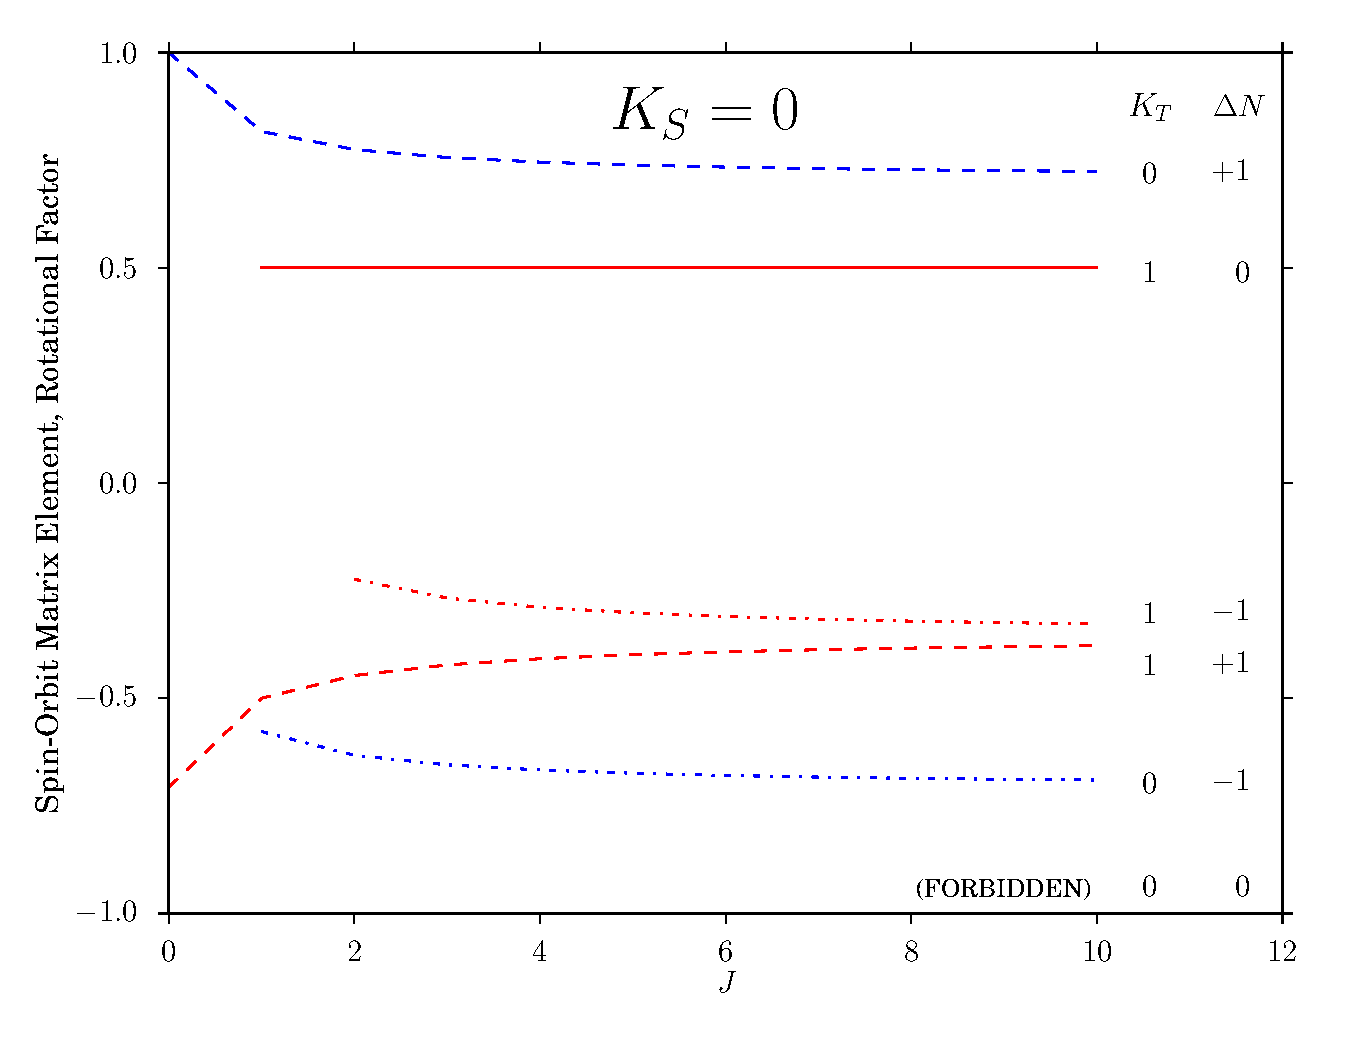
\includegraphics[width=6in]{rotational-factors-k0.pdf}
\end{figure}

%%%%%%%%%%%%%%%%%%%%%%%%%%%%%%%%%%%%%%%%%%%%%%%%%%%%%%
%%
%% END MATRIX ELEMENT FIGURE
%%
%%%%%%%%%%%%%%%%%%%%%%%%%%%%%%%%%%%%%%%%%%%%%%%%%%%%%%

The rotational selection rules between $S_1$ and $T_3$ sublevels are
perhaps best understood in terms of rotational parity.  The nonzero
rotational factors for spin-orbit matrix elements are illustrated on
energy level diagrams in Figure \ref{fig:levels-k0} for $K_T=0$
sublevels, and in Figure \ref{fig:levels-k1} for $K_T=1$ sublevels.
Figure \ref{fig:levels-k0} clearly illustrates that the $3^36^1$ and
$3^34^1$ $K_S=0$ sublevels may only mix with $K_T=0$ sublevels of the
same vibrational symmetry.  Mixing with the $F_2$ component of a
$K_T=0$ sublevel is forbidden, because the triplet rotational level is
of opposite parity.  Figure \ref{fig:levels-k1} illustrates that
triplet sublevels with $K_T=1$ contain levels of both parities for
each value of $J$ and $N$, therefore a spin-rotation level of the
correct parity is always available for mixing with a $K_S=0$ singlet
rotational level.

%%%%%%%%%%%%%%%%%%%%%%%%%%%%%%%%%%%%%%%%%%%%%%%%%%%%%%
%%
%% INSERT SINGLET-TRIPLET FIGURES HERE
%%
%%%%%%%%%%%%%%%%%%%%%%%%%%%%%%%%%%%%%%%%%%%%%%%%%%%%%%


\begin{figure}
  \caption{Diagram of spin-orbit rotational selection rules between
    the $S_1$ $3^34^1$, $3^36^1$ \Ka{0} sublevels and $T_3$ sublevels
    having $K_T=0$.  When $K_T=K_S=0$, each singlet sublevel may only
    mix with zero-order triplet sublevels of the same vibrational
    symmetry.}
  \label{fig:levels-k0}
  \centering
  \vspace{5mm}
  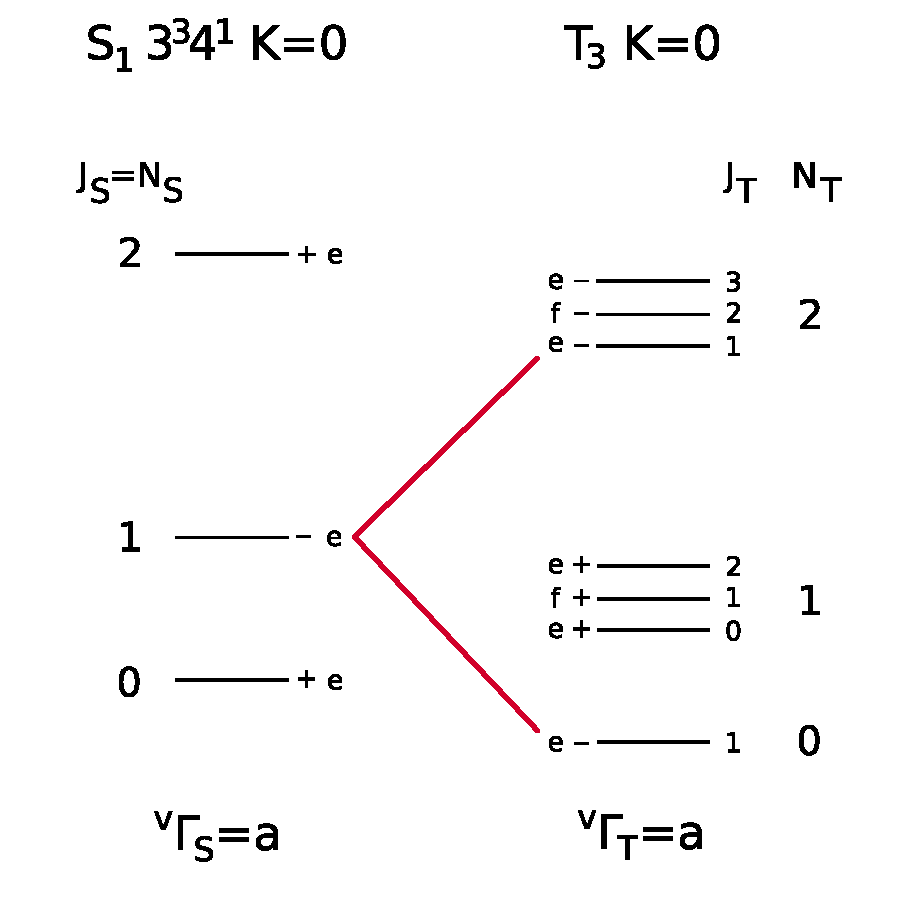
\includegraphics[width=4in,angle=90]{levels-3341}
  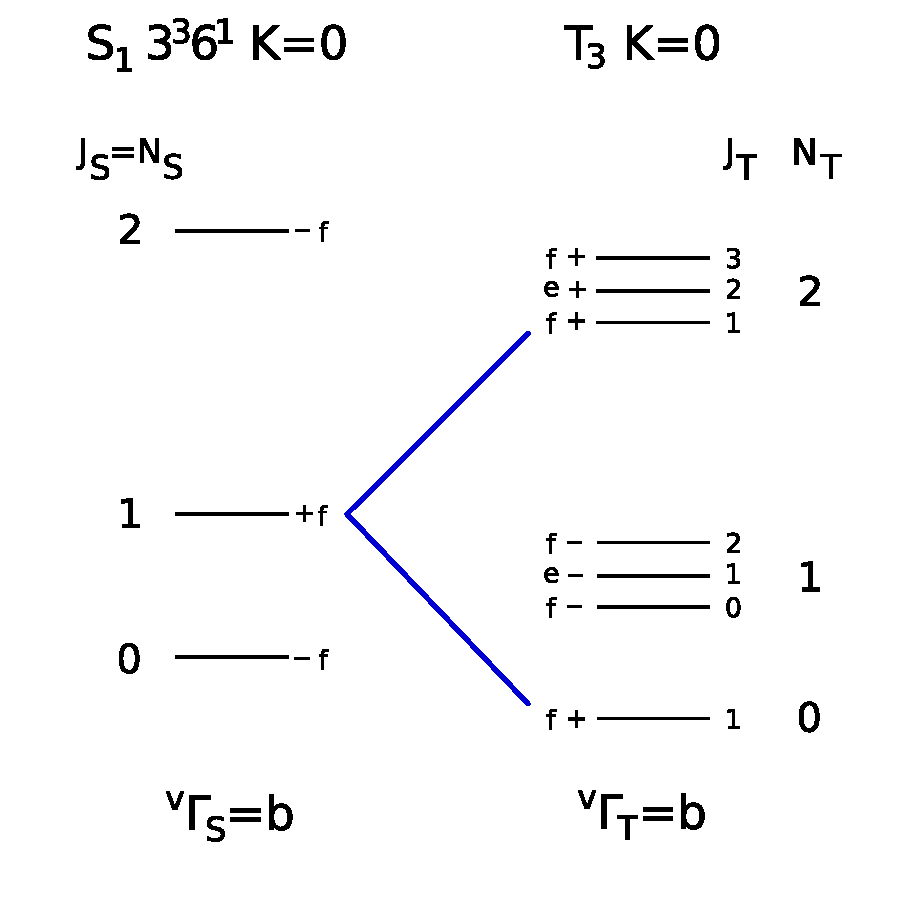
\includegraphics[width=4in,angle=90]{levels-3361}  
\end{figure}

\begin{figure}
  \caption{Diagram of spin-orbit rotational selection rules between
    the $S_1$ $3^34^1$, $3^36^1$ \Ka{0} sublevels and $T_3$ sublevels
    having $K_T=1$.  In this case, mixing is not restricted by
    vibrational symmetry, and the singlet sublevels are permitted to
    mix with the same zero-order triplet sublevel.}
  \label{fig:levels-k1}
  \centering
  \vspace{5mm}
  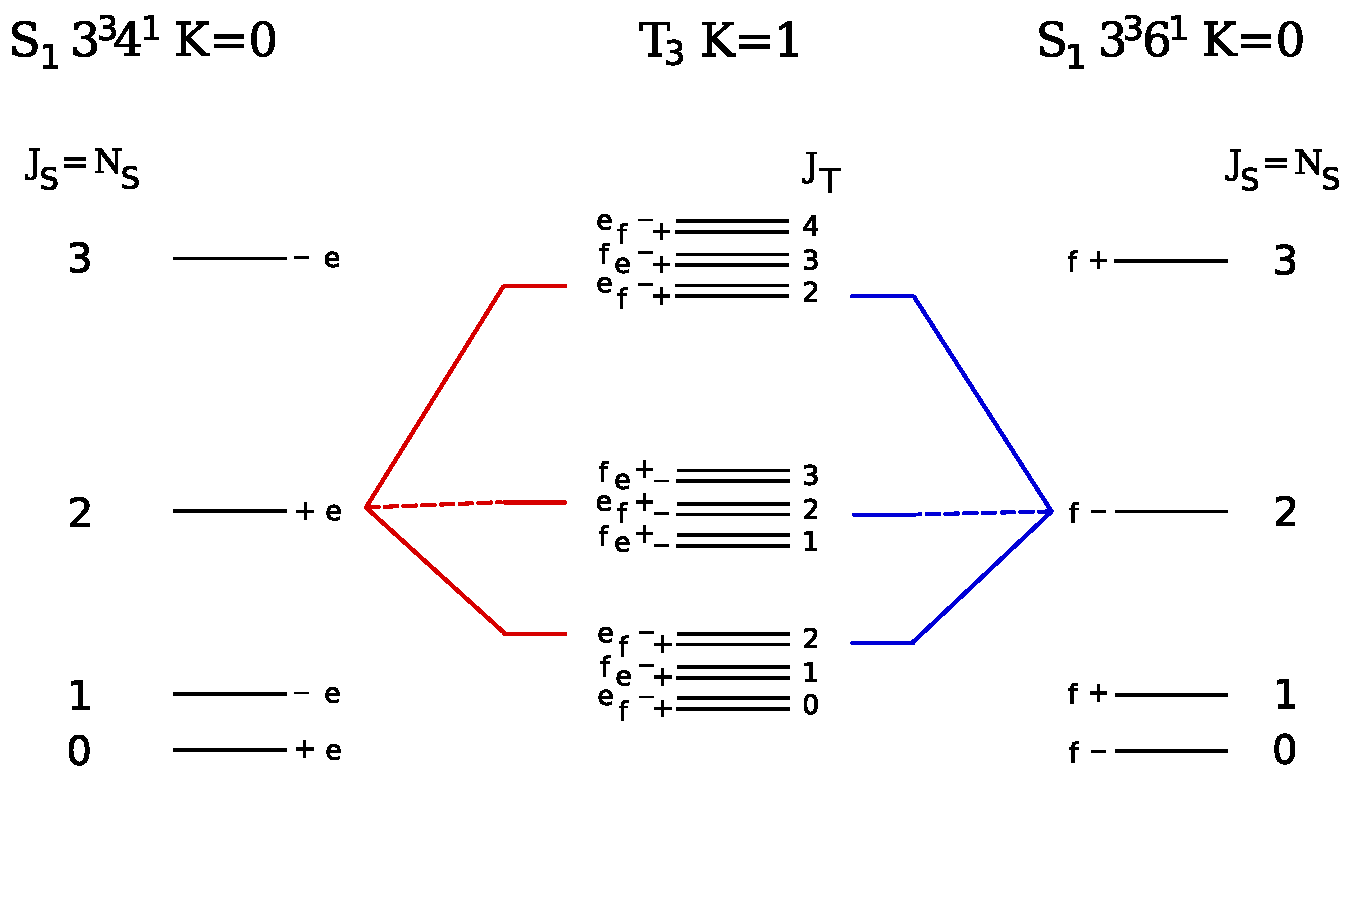
\includegraphics[width=6in,angle=90]{levels-k1}
\end{figure}

%%%%%%%%%%%%%%%%%%%%%%%%%%%%%%%%%%%%%%%%%%%%%%%%%%%%%%
%%
%% END SINGLET-TRIPLET FIGURES
%%
%%%%%%%%%%%%%%%%%%%%%%%%%%%%%%%%%%%%%%%%%%%%%%%%%%%%%%

Although specific $T_3$ doorway levels cannot be identified from our
spectra, the relative energy of $T_3$ doorways is determined from line
splittings that appear in the delayed LIF spectra of $S_1$ $3^36^1$
\Ka{0} and $3^34^1$ \Ka{0}.  The magnitudes of the spin-orbit matrix
element between the $S_1$ level and the doorway level are estimated
from the variance of the LIF spectrum.  Additionally, the allowed
vibrational symmetries of $T_3$ doorway states are discussed above in
terms of spin-orbit selection rules for $\Delta K$.





















% \TODO{Use Bryan's program to compute overlap integrals for the two bands.}

% \TODO{Show number of modes available in each symmetry as a function
%   of energy.}



\subsection{SEELEM Spectrum: \\Characterization of the local manifold of
  $T_{1,2}$ levels}

The SEELEM spectrum shows the distribution of nominal $T_{1,2}$
eigenstates that have approximately 0.25\% fractional $S_1$ character.
This specificity in SEELEM detection probability, discussed in Chapter
4.3.1, arises from the competing effects of excitation probability,
electron ejection probability and survival probability.  When the
$T_3$ doorway level is energetically distant ($\Delta E > 1$ \rcm),
the envelope of SEELEM-detectable states is not expected to exhibit
large interference effects, as observed in $S_1$ $3^3$ \Ka{1}.
Interference effects in the SEELEM spectrum result from a cross term
in the equation for SEELEM detection probability, described in Chapter
2.3.3.

Levels of the $T_1$ and $T_2$ electronic states are observed to be
extensively mixed in this energy region, evidenced by the widely
varying Land\'{e} $g$-factors observed in Zeeman Anticrossing (ZAC)
spectra \cite{dupre95a}.  (Although many of the states observed in the
ZAC experiments are nominally $S_0$, the authors rule out extensive
$S_0 \sim T_{1,2}$ mixing as the underlying cause for the widely
varying $g$-factors.  Such mixing would cause the average $g$-factor
to be approximately zero as discussed in Section 5.1 of
\cite{dupre95a}.)

We adopt a simple model, first proposed by Bixon and Jortner, to
address $T_3 \sim T_{1,2}$ mixing \cite{bixon68}.  Mixing between a
bright state and an ensemble of equally spaced dark states with
identical matrix elements results in a Lorentzian intensity envelope,
\begin{equation}
  a^2 = \frac{v^2}{\Delta E^2 + v^2}.
\end{equation}
The rigidity of $T_{1,2}$ levels in the molecule is certainly less
than that in the model, even in the limit of total mixing within each
pure sequence of states.  However, such models are shown to be
approximately correct for real systems, and in any case lend insight
into the basic mechanism at work.  We tentatively adopt this as a
zero-order model and make a comparison to the observed SEELEM spectra.

The SEELEM spectra recorded with the individual line method were fit to
Lorentzian envelopes.  To carry out the fit, the SEELEM spectrum was
first smoothed to approximately twice the average level spacing, using
a Hamming window function for convolution.  A Lorentzian profile was
fit to the smoothed spectrum using a non-linear least-squares
regression.  Figure \ref{fig:seelem-fits} shows the best-fit
Lorentzian profiles obtained for the $J'=1-5$ rotational levels of
$3^36^1$ \Ka{0}.  The Lorentzian half-width varies between 0.39 and
0.59 \rcm.

% The full width at half maximum (FWHM) of the SEELEM distribution is
% derived in Chapter 2, in terms of the $S_1 \sim T_3$ mixing angle,
% $\alpha$, and the average $T_3 \sim T_{1,2}$ matrix element,
% $H_{T_3T_{1,2}}$.  Our results led to the following formula:
% \begin{equation}
%   \text{FWHM} = 
%     \frac{2}{\sqrt{e R_m}} 
%     \left \lvert 
%       \alpha \: H_{H_{T_3T_{1,2}}}
%     \right \rvert, 
% \end{equation}
% where $R_m$ is a constant equal to the zero-order $S_1$ fluorescence
% lifetime divided by the flight time to the SEELEM detector.  The
% zero-order $S_1$ fluorescence lifetime of acetylene \astate\ is
% approximately 270 ns \cite{ochi91}.  The molecular flight time from
% the point of excitation to the SEELEM surface was measured as 309
% \microsec\ in this study.  Evaluating this equation using the average
% observed SEELEM full width at half maximum, 0.49 \rcm, we arrive at a
% value of approximately 30 \rcm\ for the product $\alpha \times
% H_{H_{T_3T_{1,2}}}$.

%%%%%%%%%%%%%%%%%%%%%%%%%%%%%%%%%%%%%%%%%%%%%%%%%%%%%%
%%
%% INSERT SEELEM FIT FIGURES
%%
%%%%%%%%%%%%%%%%%%%%%%%%%%%%%%%%%%%%%%%%%%%%%%%%%%%%%%

\begin{figure}
  \caption{Lorentzian fitting results for the $J'=1-5$ SEELEM spectra
    of the $3^36^1$ \Ka{0} sublevel.  The parameter $\Gamma$, equal to
    the half-width of the distribution, is proportional to the product
    of the $S_1 \sim T_3$ mixing angle and the average $T_3 \sim T_{1,2}$
    matrix element.  The value of $\Gamma$ is given in units of \rcm.}
  \label{fig:seelem-fits}
  \vspace{5mm}
  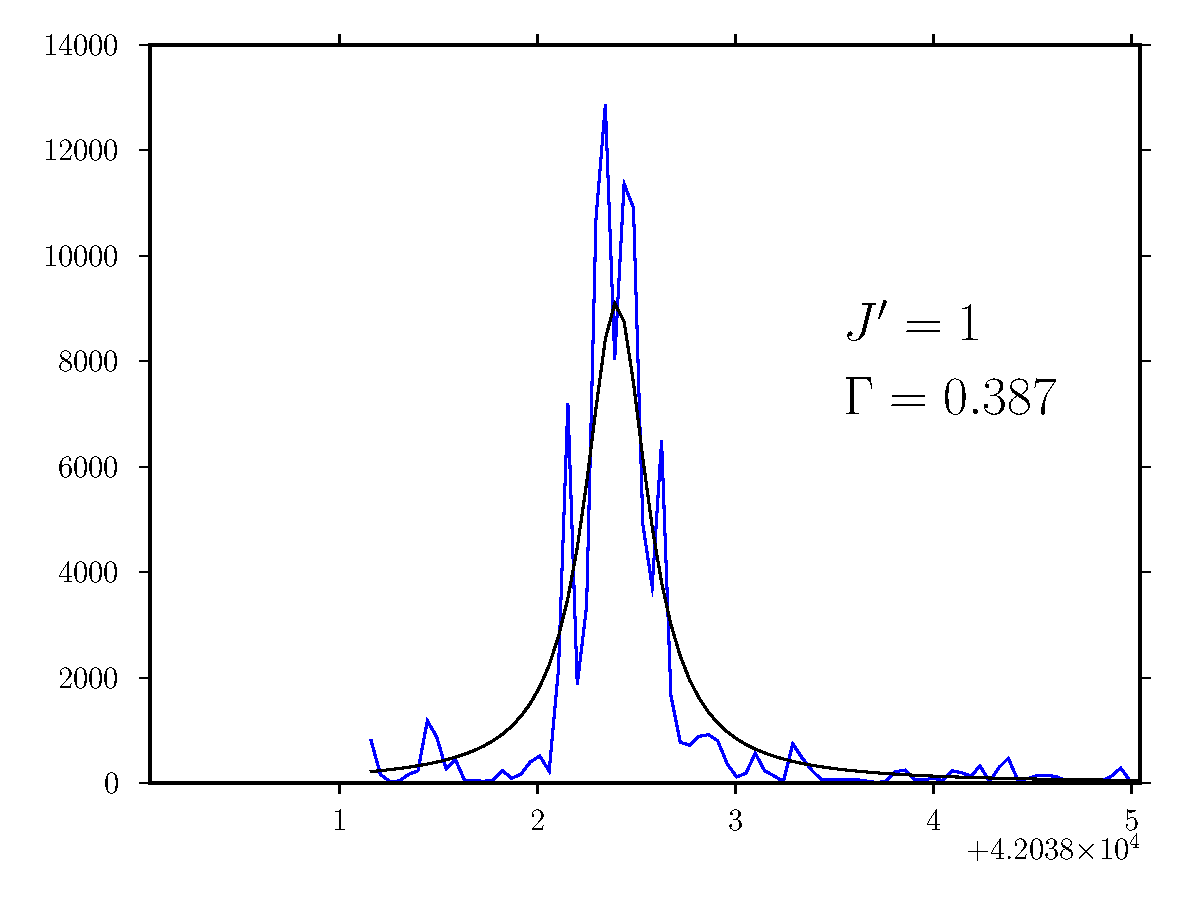
\includegraphics[width=3.2in]{3361-q1-seelemfit}
  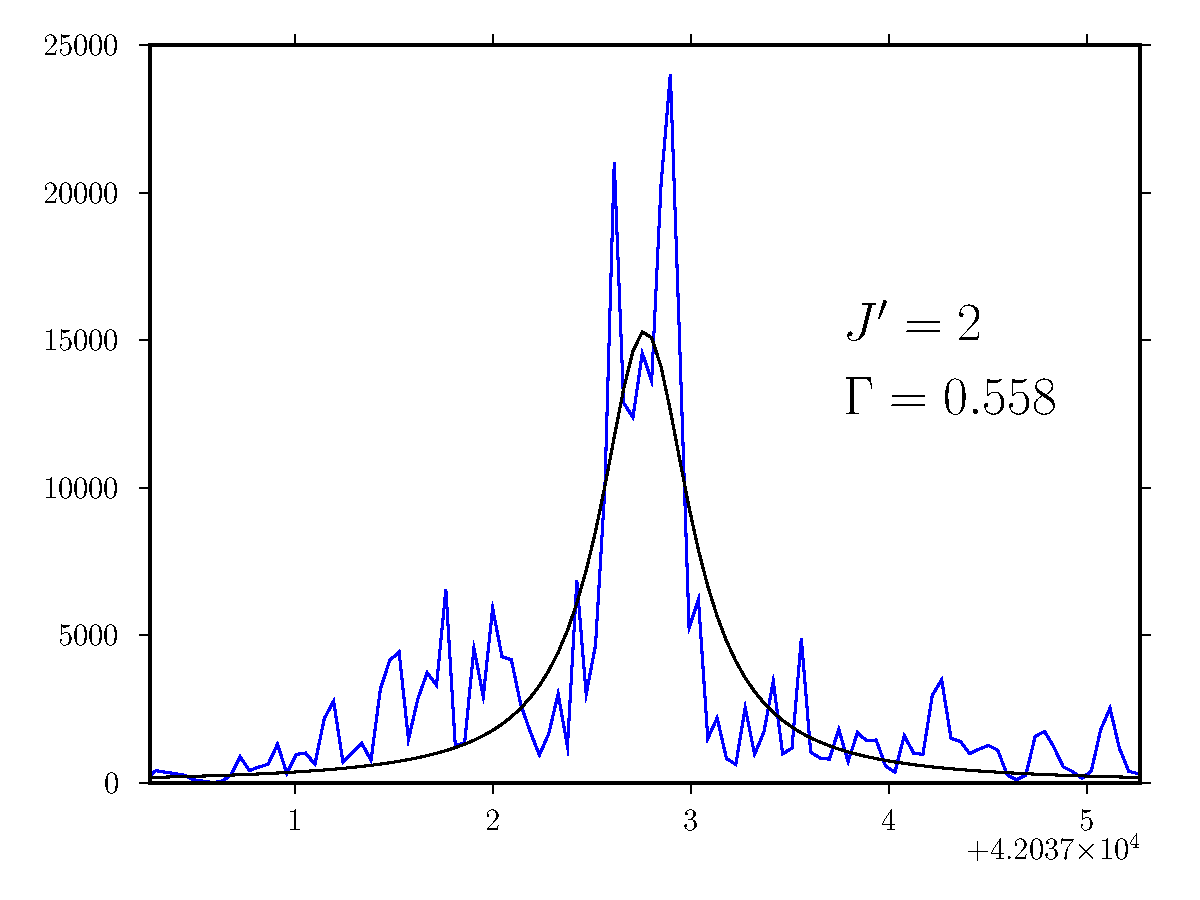
\includegraphics[width=3.2in]{3361-q2-seelemfit}
  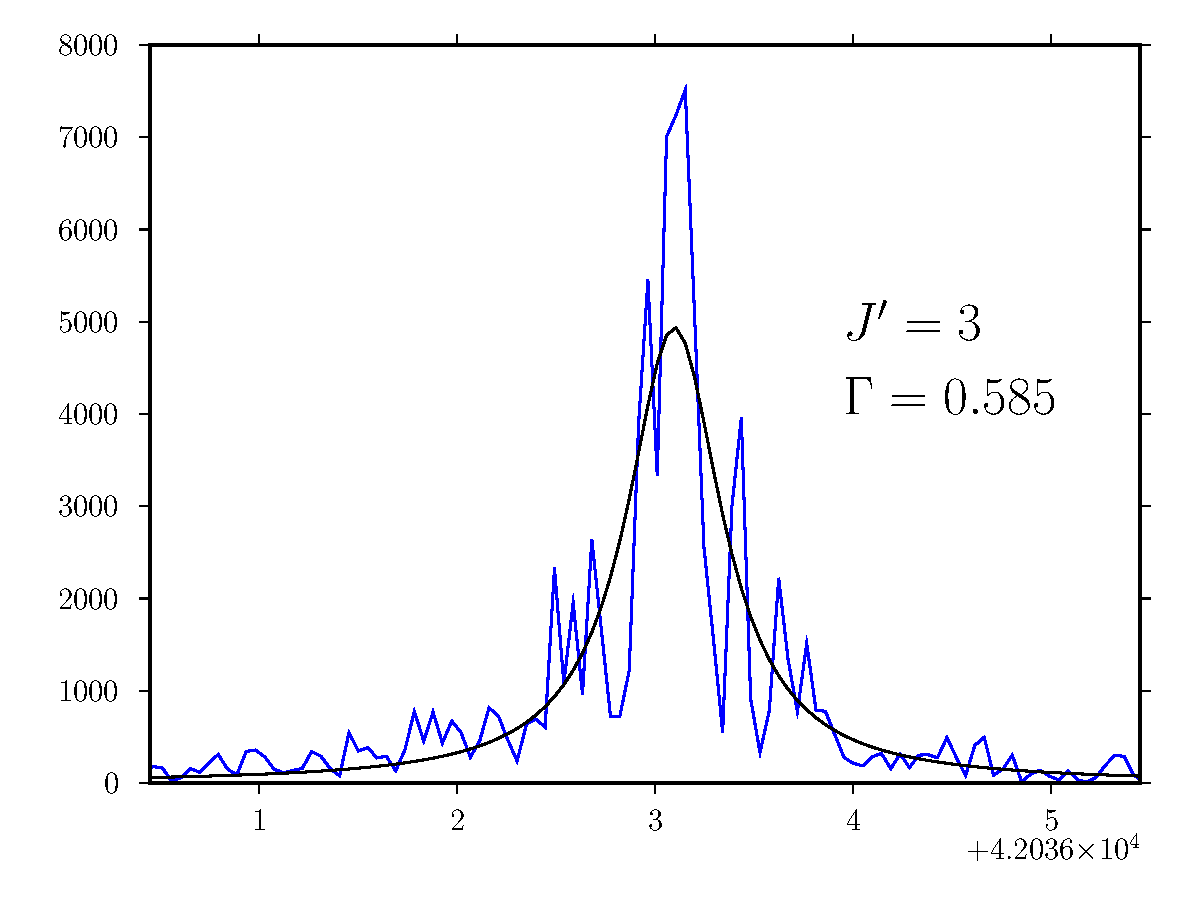
\includegraphics[width=3.2in]{3361-q3-seelemfit}
  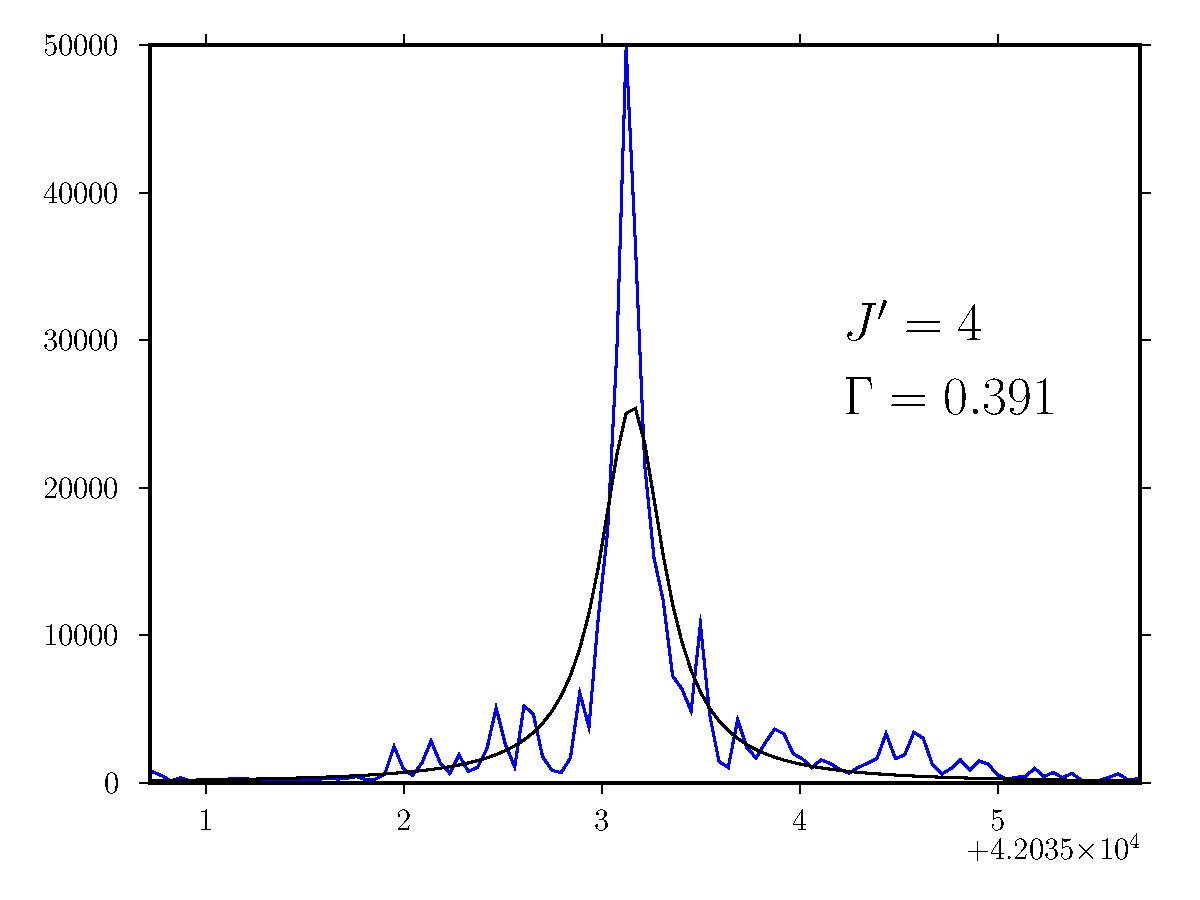
\includegraphics[width=3.2in]{3361-q4-seelemfit}
  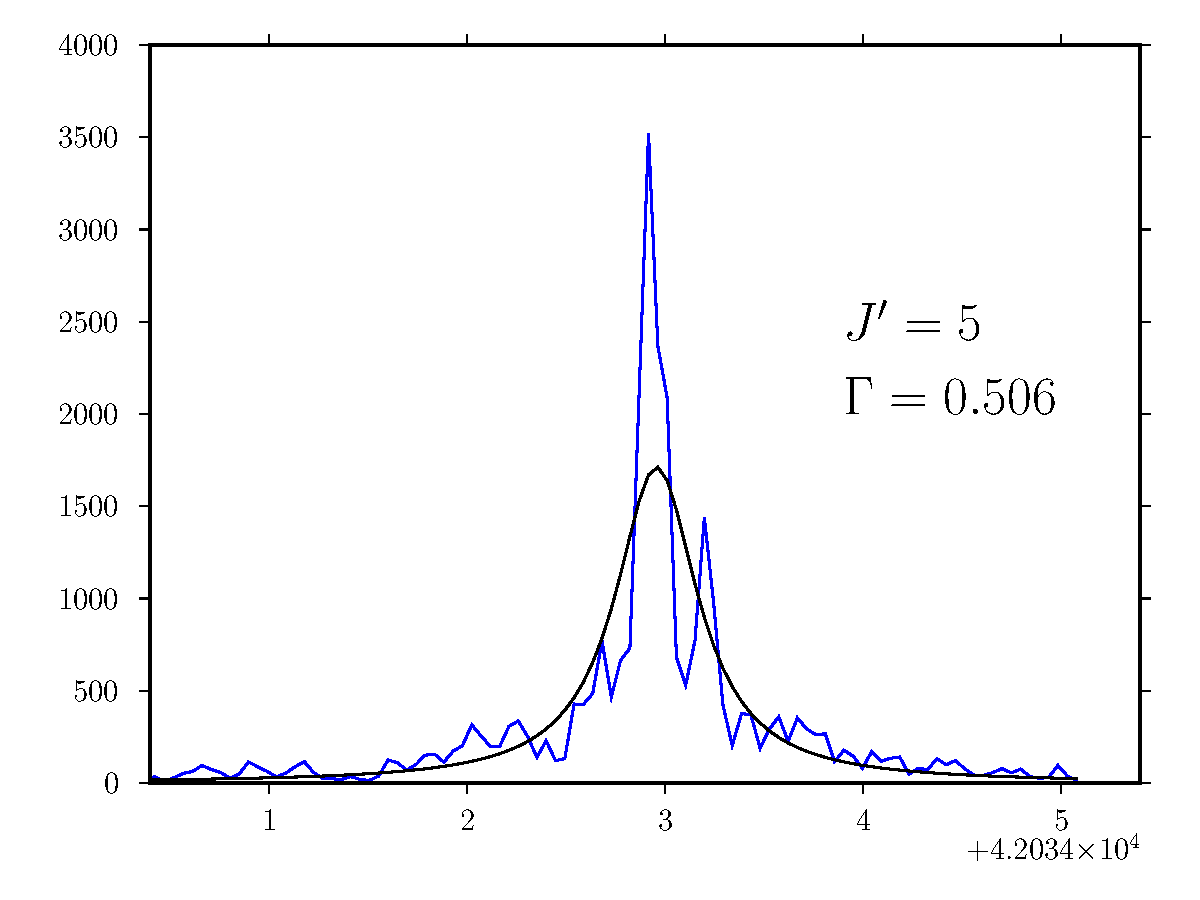
\includegraphics[width=3.2in]{3361-q5-seelemfit}
\end{figure}

%%%%%%%%%%%%%%%%%%%%%%%%%%%%%%%%%%%%%%%%%%%%%%%%%%%%%%
%%
%% END SEELEM FIT FIGURES
%%
%%%%%%%%%%%%%%%%%%%%%%%%%%%%%%%%%%%%%%%%%%%%%%%%%%%%%%

To further examine the properties of the local manifold of nominal
$T_{1,2}$ eigenstates, a reduced term value plot is prepared for the
$3^36^1$ \Ka{0} level of $S_1$ acetylene.  To construct this plot,
$S_1$ basis state rotational energies were approximated
from the early LIF spectrum by calculating the intensity-weighted
center of gravity.  The total energy of each state was reduced by an
approximate rotational term energy, $1.04 \: J'(J'+1)$.  The resulting
$S_1$ rotational energies are shown as large square markers in Figure
\ref{fig:unfold}.  The energies of nominal triplet $T_{1,2}$ levels observed in the
SEELEM spectrum are shown in the plot with small markers.  

For each SEELEM transition, a horizontal bar denotes the approximate
magnitude of the matrix element $H_{\ell m}$, according to equation
\ref{eq:approx-hlm}.  The total magnitude of the horizontal bars is
normalized separately at each value of $J'$, so comparisons are valid
only between bars appearing in the same row of the figure.  The energy
spacing and matrix elements show a remarkable uniformity, which is
expected from an extensively mixed manifold of $T_{1,2}$ levels.  The
conclusions drawn from such a figure should be treated with caution,
however, because triplet states with small matrix elements may be
obscured by others appearing with strong intensity in the SEELEM
spectrum.  \TODO{Address statistical issues surrounding this.  Mention
  distribution of matrix elements in poisson vs. goe ensembles?}

\TODO{What is the reader supposed to see in the figure? Challenge the
  reader to find any rotational series in the mess of highly-mixed
  triplet states.}

%%%%%%%%%%%%%%%%%%%%%%%%%%%%%%%%%%%%%%%%%%%%%%%%%%%%%%
%%
%% INSERT UNFOLDED INTENSITY FIGURE
%%
%%%%%%%%%%%%%%%%%%%%%%%%%%%%%%%%%%%%%%%%%%%%%%%%%%%%%%

\begin{figure}
  \caption{Reduced term value plot for the $3^36^1$ \Ka{0} level of
    $S_1$ acetylene, showing approximate $S_1$ rotational energies
    (large markers) and the energies of nominal triplet levels
    observed in the SEELEM spectrum (small markers).  For each SEELEM
    transition observed in the spectrum, a horizontal bar denotes the
    approximate spin-orbit matrix element $H_{\ell m}$.  The width of
    the horizontal bars is normalized separately for each value of
    $J'$.  The energy spacing and matrix elements show a remarkable
    uniformity, which is expected from an extensively mixed manifold
    of $T_{1,2}$ levels.}
  \label{fig:unfold}
  \centering
  \vspace{10mm}
  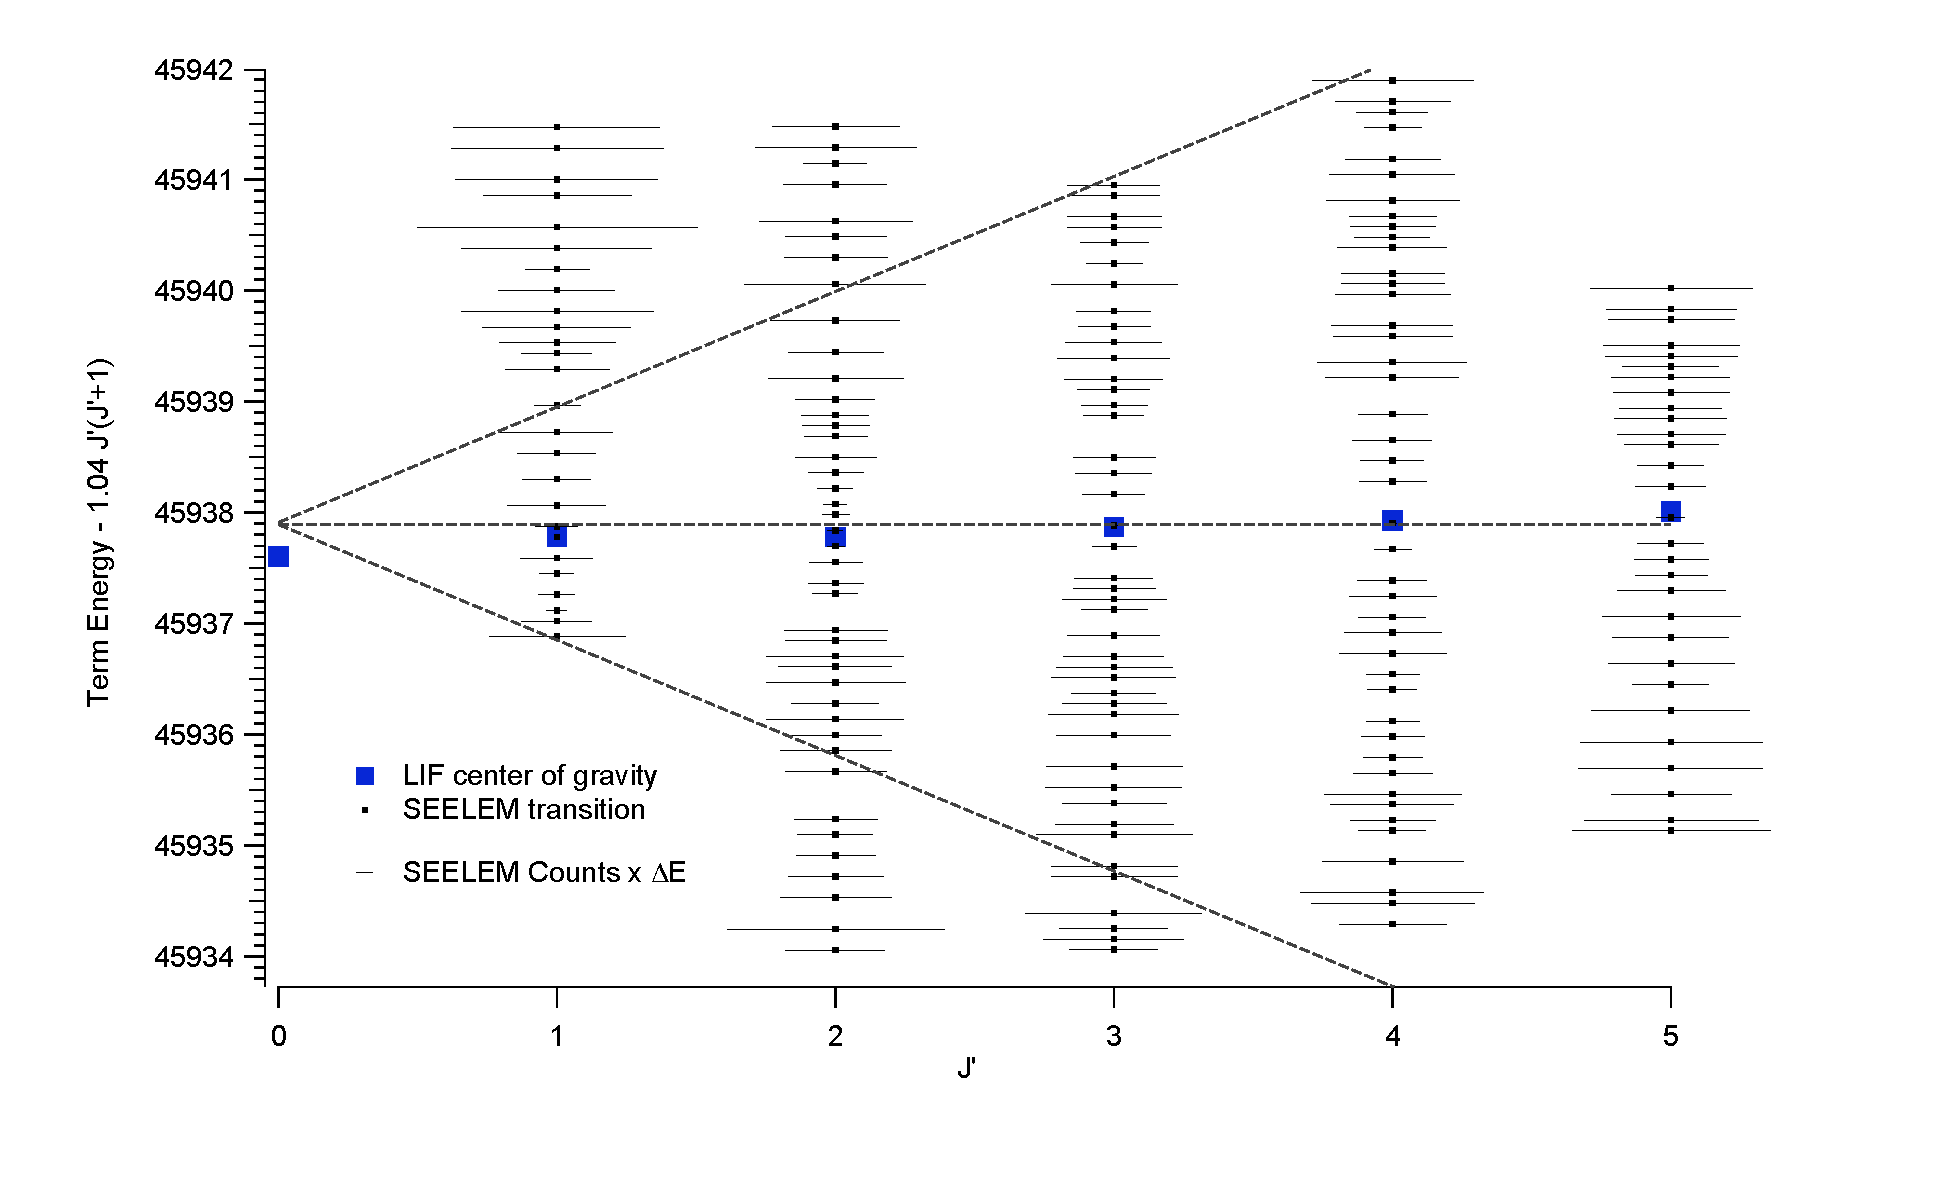
\includegraphics[width=6.2in]{redterms-3361-unfolded}
\end{figure}

%%%%%%%%%%%%%%%%%%%%%%%%%%%%%%%%%%%%%%%%%%%%%%%%%%%%%%
%%
%% END UNFOLDED INTENSITY FIGURE
%%
%%%%%%%%%%%%%%%%%%%%%%%%%%%%%%%%%%%%%%%%%%%%%%%%%%%%%%

The observation of a $J'=0$ rotational level in $3^36^1$ \Ka{0}
affords us a unique opportunity to estimate the local triplet level
density.  For a triplet vibrational sublevel with $K_T=0$ or $1$, only
a single spin component, $F_3$, is present to mix with a $J'=0$
singlet.  The vibrational symmetry of the triplet is restricted
($\Gamma_T=b$) when $K_T=0$, but unrestricted when $K_T=1$
($\Gamma_T=a$ or $b$), thus we expect to observe that the ratio of
$K_T=1$ sublevels to $K_T=0$ sublevels is 2:1.  (If Coriolis-induced
mixing is complete within the manifold of $T_{1,2}$ levels, the ratio
becomes 1:1, and the resulting state density is decreased by
approximately 24\%.)  Over an energy range of approximately 5 \rcm, we
observe approximately 26 total lines in the SEELEM and LIF spectrum.
Of these, one must be subtracted as the nominal $S_1$ bright state.
The 25 remaining lines are partitioned among triplets with $K_T=0$ and
$1$.  Counting only the expected fraction of those belonging to
$K_T=1$ sublevels, we are left with a count of approximately 16.6
levels over a range of 5 \rcm, or an observed triplet level density of
$\rho_{T_{1,2}} = 3.3$ per \rcm.  The triplet level density inferred
from this observation is in general agreement with the high-resolution
results of Drabbels and coworkers, who inferred a level density of
approximately 10 per \rcm\ from the highly fractionated LIF spectrum of
the $3^3$ \Ka{1} and $3^4$ \Ka{1} sublevels \cite{drabbels94}.  In
their observations, any of the three spin components of a triplet
sublevel with either $K_T=0, 1$ or $2$ may appear in the spectrum.  It
is therefore natural that their triplet level count should be
approximately three times higher and somewhat more uncertain than
ours.

% \POINT{Present energy levels and reduced term value plot for $3^36^1$.
%   (See p.97 of 4/2007--8/2007 notebook.)} 

% \POINT{Use $\Delta_3$ statistic, $\Sigma^2$ statistic, or Fourier
%   transform methods? (See p.65 in 11/2007--1/2008 notebook.)}

\section{Discussion}

\TODO{Discuss our estimates for matrix elements and mixing angles,
  obtained from the variance of the LIF spectrum and the Lorentzian
  width of the SEELEM spectrum.  Can we put upper/lower limits on some
  parameters?  Do our estimates agree with predictions?}

\TODO{Discuss the relative magnitudes of $S_1 \sim T_3$ mixing in
  terms of stationary phase points and seams of intersection on the
  potential surfaces.  Following the Franck-Condon principle, the
  torsional motion should promote mixing.  However, the experimental
  observations and ab initio predictions predict a stationary phase
  point close to the seam of intersection in the half-linear geometry,
  accessed by a combination of modes 3 and 6.  The ab initio
  calculations also predict that the $S_1 \sim T_3$ seam of
  intersection in the torsional coordinate occurs on the WRONG SIDE
  of the torsional well (see Figure 6 in Ventura JCP 118, 1712
  (2003)).  Why, then, do we observe some mixing in $3^34^1$ \Ka{0}?
  This is a surprising result.}

\TODO{A possible explanation is: could the observed
  singlet$\sim$triplet mixing in $3^34^1$ \Ka{0} be due primarily to
  $b$-axis Coriolis coupling with the \Ka{1} sublevel of $3^36^1$
  \Ka{1}? Derive b-axis matrix element ($\approx 1.4$ \rcm) and
  consider energy separation between the $3^34^1$ \Ka{0} level and the
  $3^36^1$ \Ka{1} sublevel ($\approx 42$ \rcm).  This leads to a
  mixing angle of about 0.03.  The observed splitting in $3^36^1$
  \Ka{1} is approximately 1 \rcm, indicating what is probably a local
  $T_3$ perturber with a matrix element of 0.5 \rcm.  Mixing with
  $3^36^1$ \Ka{1} would lead to a mixing angle of approximately 0.015
  with the $T_3$ perturber, which is not sufficient to cause 0.3 \rcm
  splittings in $3^34^1$ \Ka{0}.}

\TODO{Examine observations in terms of Josh's new acetylene
  wavefunction calculations.  The $\nu_3 \sim \nu_6$ anharmonic matrix
  element is much larger than the $\nu_3 \sim \nu_4$ matrix element,
  and provides a pathway for $T_{2,1} \leftarrow T_3 \leftarrow S_1$
  coupling.  IF the stationary phase point is in a half-linear
  geometry, the combination of modes 3 and 6 is the perfect storm to
  drive a node of the vibrational wavefunction in the right direction.
  Due to the nature of the potential well, wavefunctions with
  trans-vibration alone spread out at a 45\degrees angle to the
  stationary phase point.  One node of cis-bend is enough to ``push''
  a node of the wavefunction directly toward the half-linear turning
  point. }

\TODO{Do we see too many doorways, or do we observe the expected
  number?  The answer lies in the definition of a doorway state -- it
  is simply that level of $T_3$ with the largest mixing
  angle. Reiterate that we basically are working with a three tier
  model in the limit of low level density in the second tier.  The
  doorway model is a natural consequence of operating in this limit,
  because energy denominator effects make it likely that a single
  $T_3$ level mixes to a much greater degree than all others.
  However, there is no fundamental principle which precludes
  interaction with more than one doorway.  A single doorway model is
  simply our zero-order picture.}

\TODO{Adventurous point: why have we not, to date, observe $T_3$
  doorway levels directly, in the LIF spectrum? Could it be because
  they are too fractionated into the local manifold of $T_{1,2}$
  levels?  This would reduce their fluorescence intensity greatly, and
  cause them to appear as wide Lorentzian lineshapes in the SEELEM
  spectrum.  It seems that we may be able cite our estimation of
  coupling width in this discussion.}

\section{Conclusion}

\TODO{Write this section.}

% \section{Recycle bin}

% \emph{This spring, Adam and Hans were mapping out the non-symmetric
%   bending polyads of acetylene in IR-UV double resonance experiments.
%   During this process, they encountered a number of vibrational
%   subbands with telltale signs of singlet-triplet coupling: long
%   lifetimes, fractionation, and strong quantum beats.  With help from
%   Hans, Wilton and I were able to study a few of these bands with the
%   SEELEM detector, illuminating the metastable eigenstates connected
%   to these allowed transitions.}


% Several recent \emph{ab initio} calculations have established a
% non-planar equilibrium geometry for the $T_3$ state of acetylene.  The
% most recent claculations by Bryan Wong [\emph{JCP} 126, 184307 (2007)]
% give a torsional angle of $105^\circ$, which is well in line with the
% earlier results of Ventura \emph{et al} [\emph{JCP} 118, 1702 (2003)].
% Since the $T_3$ state is known to play a role in coupling the $S_1$
% state to the bath of metastable $T_{1,2}$ states, we wish to
% investigate vibrational motions that may promote coupling between
% $S_1$ and $T_3$.  In particular, we are interested in the torsional
% mode $\nu_4'$, which twists the molecule out of a planar geometry.

% However, the two non-symmetric bending modes $\nu_4'$ and $\nu_6'$ are
% strongly coupled by Darling-Dennison and a-type Coriolis interactions.
% Our recent submission to \emph{JPC A} contains an overview of these
% effects as they relate to singlet-triplet coupling.  Anthony Merer and
% the Singlets understand these couplings very well and are now in the
% process of writing what is sure to be the classic paper on this topic.

% We wanted to ivestigate subbands where these effects are not present.

% both $K=0$ subbands show signs of strong singlet-triplet mixing.

% This particular polyad has been studied before. The most relevant
% paper is Nami and Soji's study of Zeeman quantum beats in the $3^3 B^1
% K=1$ subbands [\emph{CPL} 348, 53 (2001)].  They observe strong
% splitting and Zeeman quantum beats in the $3^3 6^1$ band, but not in
% the band involving torsion.

% Our results follow.  The first two spectra give an overview of both
% bands.  We use overlapping transitions of $J'=1-6$ in the Q-branch of
% the intermediate state to take spectra that \emph{look} like
% one-photon spectra.  Unlike Nami and Soji's observations in the $K=1$
% levels, we observe splittings and strong SEELEM signal in the $3^3
% 4^1$ band when $K=0$.

% The major advantage of working in double resonance is of course the
% ability to simplify the spectrum.  This is especially beneficial for
% SEELEM experiments, because the manifold of metastable states
% borrowing intensity from one rotational level often overlaps with that
% of the next.  We examined each rotational level in turn for $3^3 6^1$,
% collecting SEELEM data for each rotational level of the bright state
% without overlap from neighboring levels.  Since the spin-orbit
% operator is diagonal in $J$, we get this quantum number for free when
% we examine one rotational transition at a time.

% The SEELEM signals for these transitions are the strongest we have
% ever recorded for acetylene.  Even the ``weak'' intensity regions are
% full of well-resolved lines, as illustrated in a close-up of our data
% from $J'=4$.


\bibliography{master}
\bibliographystyle{plain}
\end{document}
% LocalWords:  sublevel initio Condon Mizoguchi Zeeman sublevels Yamakita Cui
% LocalWords:  publised Morokuma deperturbation
